%%%%%%%%%%%%%%%%%%%%%%%%%%%%%%%%%%%%%%%%%%%%%%%%%%%%%%%%%%%%
%%% ELIFE ARTICLE TEMPLATE
%%%%%%%%%%%%%%%%%%%%%%%%%%%%%%%%%%%%%%%%%%%%%%%%%%%%%%%%%%%%
%%% PREAMBLE 
\documentclass[9pt,lineno,final]{elife}
% Use the onehalfspacing option for 1.5 line spacing
% Use the doublespacing option for 2.0 line spacing
% Please note that these options may affect formatting.
% Additionally, the use of the \newcommand function should be limited.

% Article specific functions
\newcommand{\pKa}{p\textit{K}\textsubscript{a}}
\newcommand{\poKa}{p\textsubscript{o}\textit{K}\textsubscript{a}}
\newcommand{\logD}{log~\textit{D}}
\newcommand{\logP}{log~\textit{P}}


\usepackage{lipsum} % Required to insert dummy text
\usepackage[version=4]{mhchem}
%\usepackage{siunitx}
%\DeclareSIUnit\Molar{M}
%\usepackage[colorinlistoftodos]{todonotes}
\usepackage[color=green!30, textsize=small]{todonotes}
\usepackage{gensymb}
\usepackage{mhchem}
\usepackage{wrapfig}
\usepackage{booktabs}

\usepackage[flushleft]{threeparttable}
%\usepackage[table,xcdraw]{xcolor}
%\usepackage{longtable} % for tables that are longer than one page
\usepackage{float}

% some tint of orange
\definecolor{tangelo}{rgb}{0.98, 0.3, 0.0}
% var for storing a box size
\newsavebox{\measurebox}

% Hidden table column
%\newcolumntype{H}{>{\setbox0=\hbox\bgroup}c<{\egroup}@{}}

% For having Supplemantary Information Section in the same document
\newcommand{\beginsupplement}{%
        \setcounter{table}{0}
        \renewcommand{\thetable}{S\arabic{table}}%
        \setcounter{figure}{0}
        \renewcommand{\thefigure}{S\arabic{figure}}%
     }
     
% To have landscape pages
\usepackage{pdflscape}

% For color coded to-do and comment bubbles
\newcommand{\todoMI}[1]{\todo[inline, author=MI, color=blue!20]{ #1}}


%%%%%%%%%%%%%%%%%%%%%%%%%%%%%%%%%%%%%%%%%%%%%%%%%%%%%%%%%%%%
%%% ARTICLE SETUP
%%%%%%%%%%%%%%%%%%%%%%%%%%%%%%%%%%%%%%%%%%%%%%%%%%%%%%%%%%%%
\title{Accuracy of macroscopic and microscopic \pKa{} predictions of small molecules evaluated by the SAMPL6 blind prediction challenge}

\author[1,2*]{Mehtap Işık (ORCID: \href{http://orcid.org/0000-0002-6789-952X}{0000-0002-6789-952X})}
\author[1,3]{Ari\"{e}n S. Rustenburg (ORCID: \href{http://orcid.org/0000-0002-3422-0613}{0000-0002-3422-0613})}
\author[1,4]{Andrea Rizzi (ORCID: \href{https://orcid.org/0000-0001-7693-2013}{0000-0001-7693-2013})}
\author[6]{M. R. Gunner} % Marilyn wants to be "M. R. Gunner"
\author[5]{David L. Mobley (ORCID: \href{http://orcid.org/0000-0002-1083-5533}{0000-0002-1083-5533})}
\author[1]{John D. Chodera (ORCID: \href{http://orcid.org/0000-0003-0542-119X}{0000-0003-0542-119X})}

\affil[1]{Computational and Systems Biology Program, Sloan Kettering Institute, Memorial Sloan Kettering Cancer Center, New York, NY 10065, United States}
\affil[2]{Tri-Institutional PhD Program in Chemical Biology, Weill Cornell Graduate School of Medical Sciences, Cornell University, New York, NY 10065, United States}
\affil[3]{Graduate Program in Physiology, Biophysics, and Systems Biology, Weill Cornell Medical College, New York, NY 10065, United States}
\affil[4]{Tri-Institutional PhD Program in Computational Biology and Medicine, Weill Cornell Graduate School of Medical Sciences, Cornell University, New York, NY 10065, United States}
\affil[5]{Department of Pharmaceutical Sciences and Department of Chemistry, University of California,
Irvine, Irvine, California 92697, United States}
\affil[6]{Department of Physics, City College of New York, New York NY 10031}

\corr{mehtap.isik@choderalab.org}{MI}

%%%%%%%%%%%%%%%%%%%%%%%%%%%%%%%%%%%%%%%%%%%%%%%%%%%%%%%%%%%%
%%% ARTICLE START
%%%%%%%%%%%%%%%%%%%%%%%%%%%%%%%%%%%%%%%%%%%%%%%%%%%%%%%%%%%%

\begin{document}

\maketitle

%%%%%%%%%%%%%%%%%%%%%%%%%%%%%%%%%%%%%%%%%%%%%%%%%%%%%%%%%%%%
% Abstract
%%%%%%%%%%%%%%%%%%%%%%%%%%%%%%%%%%%%%%%%%%%%%%%%%%%%%%%%%%%%
\begin{abstract}

Acid dissociation constant (\pKa{}) prediction is a prerequisite for predicting many other properties of small molecules such as protein-ligand binding affinity, distribution coefficient (\logD{}), membrane permeability, and solubility due to the necessity of predicting relevant protonation states and the free energy penalty of each state. 
SAMPL6 \pKa{} Challenge was the first time that a separate challenge was conducted for evaluating \pKa{} predictions as a part of SAMPL. 
It was motivated by the inaccuracies observed in prior physical property prediction challenges, such as SAMPL5 \logD{} Challenge, caused by protonation state and \pKa{} prediction issues. 
The goal of the \pKa{} challenge was to elucidate the performance of contemporary \pKa{} prediction methods for drug-like molecules. 
The challenge set was composed of 24 kinase inhibitor fragment-like small molecules and some of them were multiprotic. 
11 research groups contributed blind prediction sets of 37 \pKa{} prediction methods. 
Four widely used \pKa{} prediction methods that were missing from blind predictions were added as reference methods to challenge analysis. Collecting both microscopic and macroscopic \pKa{} predictions allowed in-depth evaluation of \pKa{} prediction performance. 
This article highlights deficiencies of typical \pKa{} prediction evaluation approaches when the difference between microscopic and macroscopic \pKa{}s is ignored and suggests more stringent evaluation criteria for microscopic and macroscopic \pKa{} predictions guided by the available experimental data. 
Top-performing submissions for macroscopic \pKa{} predictions achieved RMSE of 0.7-1.0 units and included both quantum-mechanical and empirical approaches. 
These predictions included less than 8 extra/missing macroscopic \pKa{}s for the set of 24 molecules. 
A large number of submissions had RMSE spanning 1-3 \pKa{} units. Molecules with sulfur-containing heterocycles, iodo, and bromo groups suffered from less accurate \pKa{} predictions on average considering all methods evaluated. 
For a subset of molecules, the available NMR-based dominant microstate sequence data was utilized to elucidate dominant tautomer prediction errors of microscopic \pKa{} predictions which was prominent for charged tautomers. 
SAMPL6 \pKa{} Challenge demonstrated the need for improving \pKa{} prediction methods for drug-like molecules, especially for challenging moeities and multiprotic molecules. 
The level of \pKa{} prediction inaccuracy observed in this challenge has potential to be detrimental to the performance of protein-ligand binding affinity predictions in two ways: (1) errors in predicted dominant charge and tautomeric state and (2) errors in the calculation of free energy correction for minor and multiple protonation states of the ligand.
\end{abstract}

%%%%%%%%%%%%%%%%%%%%%%%%%%%%%%%%%%%%%%%%%%%%%%%%%%%%%%%%%%%%
% Keywords and Abbreviations
%%%%%%%%%%%%%%%%%%%%%%%%%%%%%%%%%%%%%%%%%%%%%%%%%%%%%%%%%%%%
\subsection{Keywords}
SAMPL $\cdot$ blind prediction challenge $\cdot$ acid dissociation constant $\cdot$ \pKa{} $\cdot$ small molecule $\cdot$ macroscopic \pKa $\cdot$ microscopic \pKa  $\cdot$ macroscopic protonation state $\cdot$ microscopic protonation state

\subsection{Abbreviations}
\begin{description}
\item[SAMPL] Statistical Assessment of the Modeling of Proteins and Ligands
\item[\pKa]  --${\log_{10}}$ acid dissociation equilibrium constant 
\item[SEM] Standard error of the mean
\item[RMSE] Root mean squared error
\item[MAE] Mean absolute error
\item[{$\tau$}] Kendall's rank correlation coefficient (Tau)
\item[R\textsuperscript{2}] Coefficient of determination (R-Squared)
\end{description}


%%%%%%%%%%%%%%%%%%%%%%%%%%%%%%%%%%%%%%%%%%%%%%%%%%%%%%%%%%%%
% Introduction
%%%%%%%%%%%%%%%%%%%%%%%%%%%%%%%%%%%%%%%%%%%%%%%%%%%%%%%%%%%%
\section{Introduction}

The acid dissociation constant (\pKa{}) describes the protonation state equilibrium of a molecule given pH. 
Predicting \pKa{} is a prerequisite for predicting many other properties of small molecules such as protein-ligand binding affinity, distribution coefficient (\logD{}), membrane permeability, and solubility. 
Computer-aided drug design efforts include assessing properties of virtual molecules to guide synthesis and prioritization decisions. 
In such cases an experimental \pKa{} measurement is not possible. Therefore, accurate computational \pKa{} prediction methods are required.

For a monoprotic weak acid (HA) or base (B) dissociation equilibria shown in Equation 1, the acid dissociation constant is expressed as in Equations 2 or its common negative logarithmic form as in Equation 3. 
The ratio of ionization states can be calculate with HHenderson-Hasselbalch equations shown in Equation 4. 

\begin{equation}
HA \rightleftharpoons A^- + H^+ \;\;\;\;\; BH^+ \rightleftharpoons B + H^+
\end{equation}

\begin{equation}
K_a = \frac{[A^-][H^+]}{[HA]}\;\;\;\;\;K_a = \frac{[B][H^+]}{[B^+]} 
\end{equation}


\begin{equation}
pK_a = -\log_{10}{K_a}
\end{equation}


\begin{equation}
pH = pK_a + \log_{10}{\frac{[A^-]}{[HA]}}\;\;\;\;\;pH = pK_a + \log_{10}{\frac{[B]}{[BH^+]}}
\end{equation}


Ionizable sites are found often in drug molecules and influence their pharmaceutical properties including target affinity, ADME/Tox, and formulation properties~\citep{Manallack:2013:ChemSocRev}. 
Drug molecules with titratable groups can exist in many different charge and protonation states based on the pH of the environment. 
We rely on \pKa{} values to determine in which charge and protonation states the molecules exists and relative populations of these states. 
The pH of the human gut ranges between 1-8 and 74\% of approved drugs can change ionization states withing this physiological pH range~\citep{Manallack:2013:ChemMedChema} and because of this \pKa{} values of drug molecules provides essential information about their physicochemical and pharmaceutical properties. 
A wide distribution of acidic and basic \pKa{} values, ranging from 0 to 12, have been observed in approved drugs~\citep{Manallack:2013:ChemMedChema, Manallack:2013:ChemSocRev}.

Small molecule \pKa{} predictions influence computational protein-ligand binding affinities in multiple ways. 
Errors is \pKa{} predictions can cause modeling the wrong charge, protonation, and tautomerization states which affect hydrogen bonding opportunities and charge distribution of the ligand.
The prediction of the dominant protonation state and relative population of minor states in aqueous medium is dictated by the \pKa{} values. 
The relative free energy of different protonation states in the aqueous state is a function of \pKa{} and pH, it contributes to the overall protein-ligand affinity in the form of a free energy penalty of reaching higher energy protonation states~\citep{deOliveira:2019:J.Chem.TheoryComput.}.

Drug-like molecules present difficulties for \pKa{} prediction compared to simple monoprotic molecules. 
Drug-like molecules are frequently multiprotic, have large conjugated systems, heterocycles, tautomerization. In addition that larger molecules with conformational flexibility can have intramolecular hydrogen bonding which shifts \pKa{} values. These shifts could be real or modeling artifacts due to collapsed conformations caused by deficiencies in solvation models. Yet predicting \pKa{}s of drug-like molecules accurately is a prerequisite for computational drug discovery and design.

The definition of \pKa{} diverges into two for multiprotic molecules: macroscopic \pKa{} and microscopic \pKa{}~\citep{Darvey:1995:Biochem.Educ., Bodner:1986:J.Chem.Educ., Murray:1995:Anal.Chem.}. 
Macroscopic \pKa{} describes the equilibrium dissociation constant between different charged states of the molecule. 
Each charge state can be composed of multiple tautomers. Macroscopic \pKa{} is about the deprotonation of the molecule, not a particular titratable group. 
Microscopic \pKa{} describes the acid dissociation equilibrium between individual tautomeric states of different charges. 
We refer to collection of all tautomeric states of different macroscopic states (charge states) as microscopic states. 
Microscopic \pKa{} value defined between two microstates captures the deprotonation of a single titrable group with a fixed background protonation state of other titratable groups. 
In molecules with multiple titratable groups, the protonation state of one group can affect the proton dissociation propensity of another functional group, therefore the same titratable group may have different microscopic \pKa{} values based on the protonation state of the rest of the molecule.
Different experimental methods capture different definitions of \pKa{}s as explained in more detail in this prior publication~\citep{Isik:2018:J.Comput.AidedMol.Des.}. 
Most common \pKa{} measurement techniques such as potentiometric and spectrophotometric methods measure macroscopic \pKa{}s while NMR measurements can determine microscopic \pKa{}s and microstate populations. 
Therefore, it is important to pay attention to the source and definition of \pKa{} values to interpret their meaning correctly. 
Computational methods can predict both microscopic and macroscopic \pKa{}s. While microscopic \pKa{} predictions are more informative for determining relevant microstates/tautomers of a molecule and their relative free energies, computing predicted macroscopic \pKa{}s is useful for direct comparison of methods to more common macroscopic experimental measurements. In this paper, we explore approaches to assess the performance of both macroscopic and microscopic \pKa{} predictions, taking advantage of available experimental data.



%%%
\subsection{Motivation for a blind \pKa{} challenge}

SAMPL (Statistical Assessment of the Modeling of Proteins and Ligands) is a series of annual computational prediction challenges for the computational chemistry community. The goal of SAMPL is evaluate to current performance of the models and to bring the attention of quantitative biomolecular modeling field on major issues that limit the accuracy of protein-ligand binding models.

SAMPL Challenges that focus on different physical properties so far have assessed intermolecular binding models of various protein-ligand and host-guest systems, solvation models to predict hydration free energies and distribution coefficients. 
Potantial benefits of these challenges are motivating improvement computational methods and revealing unexpected contributors to error by focusing on interesting test systems. 
SAMPL Challenges have demonstrated the effects of force field accuracy, sampling issues, solvation modeling defects, and tautomer/protonation state predictions on protein-ligand binding predictions.  

During the SAMPL5 \logD{} Challenge, the performance of cyclohexane-water \logD{} predictions were lower than expected and accuracy suffered when protonation states and tautomers were not taken into account~\citep{Pickard:2016:J.Comput.AidedMol.Des., Bannan:2018:J.Comput.AidedMol.Des.}. 
With the motivation of deconvoluting the different sources of error contributing to the large errors observed in the SAMPL5 \logD{} Challenge, we organized separate of \pKa{} and \logP{} challenges in SAMPL6~\citep{Isik:2018:J.Comput.AidedMol.Des., Isik:2020:J.Comput.AidedMol.Des., Isik:2020:J.Comput.AidedMol.Des.a}. For this iteration of the SAMPL challenge, we have taken one step back and isolated just the problem of predicting aqueous protonation states. 

This is the first time a blind \pKa{} prediction challenge has been fielded as part of SAMPL. 
In this first iteration of the challenge, we aimed to assess the performance of current \pKa{} prediction methods for drug-like molecules, investigate potential causes of inaccurate \pKa{} estimates, and determine how much current level of expected accuracy might impact protein binding affinity predictions. 
In binding free energy predictions, any error in predicting the free energy of accessing a minor aqueous protonation state of ligand that contributes to the complex formation will directly add to the error in the predicted binding free energy. 
Similarly for \logD{} predictions, inaccurate prediction aqueous protonation state that contribute partitioning between phases or prediction of relative free energy of these states will be detrimental to the accuracy of transfer free energy predictions.

%%%
\subsection{Approaches to predict small molecule \pKa{}s}

\todo[inline]{Overview of kinds of pKa prediction methods available  (ML, QM, empirical methods ... }


%%%%%%%%%%%%%%%%%%%%%%%%%%%%%%%%%%%%%%%%%%%%%%%%%%%%%%%%%%%%
% Methods
%%%%%%%%%%%%%%%%%%%%%%%%%%%%%%%%%%%%%%%%%%%%%%%%%%%%%%%%%%%%
\section{Methods}

%%%
\subsection{Design and logistics of the SAMPL6 \pKa{} Challenge}

\begin{figure}
\begin{center}
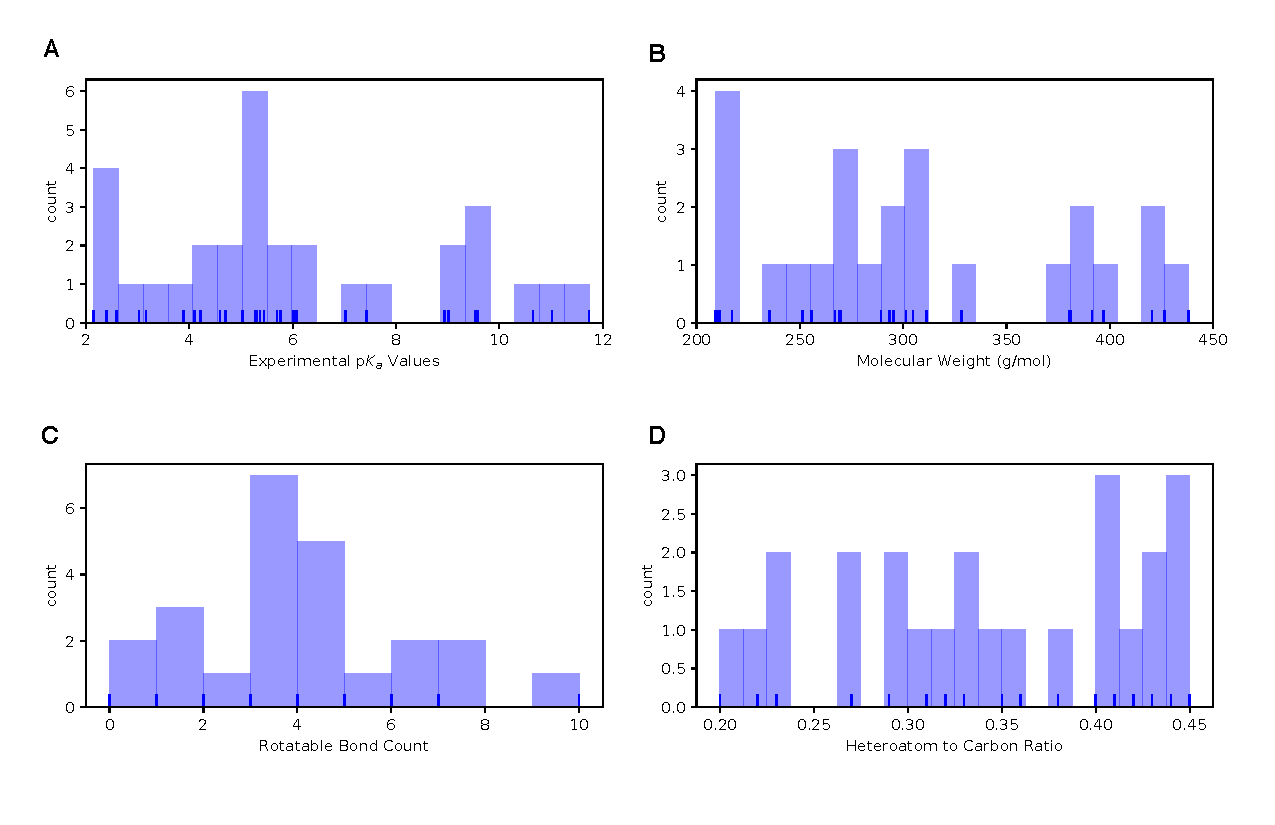
\includegraphics[width=1.0\linewidth]{figures/distribution_of_molecular_properties.pdf}
\caption{{\bf Distribution of molecular properties of 24 compounds in SAMPL6 \pKa{} Challenge.} {\bf A} Histogram of spectrophotometric \pKa{} measurements collected with Sirius T3 ~\cite{Isik:2018:J.Comput.AidedMol.Des.}. Overlayed carpet plot indicates the actual values. Five compounds have multiple measured \pKa{}s in the range of 2-12. {\bf B} Histogram of molecular weights of compounds in SAMPL6 set. Molecular weights were calculated by neglecting counter ions. {\bf C} Histogram of the number of non-terminal rotatable bonds in each molecule. {\bf D} The histogram of the ratio of heteroatom (non-carbon heavy atom) count to the number of carbon atoms.
}
\label{fig:dist_mol_prop}
\end{center}
\end{figure}

The SAMPL6 \pKa{} Challenge was conducted as a blind prediction challenge focus on predicting aqueous \pKa{} value of 24 small molecules that resemble fragments of kinase inhibitors. 
The compound selection process was described in depth in the prior publication reporting SAMPL6 \pKa{} Challenge experimental data collection~\citep{Isik:2018:J.Comput.AidedMol.Des.}.
The distribution of molecular weights, experimental \pKa{} values, number of rotatable bonds, and heteroatom to carbon ratio are depicted in Fig.~\ref{fig:dist_mol_prop}. The challenge molecule set was composed of 17 small molecules with limited flexibility (less than 5 non-terminal rotatable bonds) and 7 molecules with 5-10 non-terminal rotatable bonds. 
The distribution of experimental \pKa{} values ranged between 2-12 and roughly uniform. 
2D representations of all compounds were provided in Fig.~\ref{fig:molecules_with_MAE_of_all_methods}. 
Drug-like molecules are often larger and more complex than the ones used in this study, however, aimed for the

The dataset composition and details of the \pKa{} measurement technique, except the identity of the small molecules, were announced about a month before the challenge start time. 
Experimental macroscopic \pKa{} measurements were collected with spectrophotometric method of Sirius T3, at room temperature in ionic strength-adjusted water with 0.15 M KCl~\citep{Isik:2018:J.Comput.AidedMol.Des.}. 
The instructions for participation and the identity of the challenge molecules were released at the challenge start date (October 25, 2017). 
A table of molecule IDs (in the form of SM\#\#) and	their canonical isomeric SMILES was provided as input.
Blind prediction submissions were accepted until January 22, 2018. 

Following the conclusion of the blind challenge, the experimental data was made public on January 23, 2018. The SAMPL organizers and participants gathered at the Second Joint D3R/SAMPL Workshop, at UC San Diego, La Jolla, CA on February 22-23, 2018 to share results.
The workshop aimed to create an opportunity for participants to have discussions, evaluate the results and lessons of the challenge together. 
The participants reported their results and their own evaluations in the special issue of the Journal of Computer-Aided Molecular Design~\citep{JCAMD_special_issue_pKa}. 

In this first iteration of \pKa{} prediction challenge we were not sure what was the best way to capture all necessary information related to \pKa{} predictions. Our aim was to directly evaluate macroscopic \pKa{} predictions comparing them to experimental macroscopic \pKa{} values and to use collected microscopic \pKa{} prediction data for more in-depth diagnostics of method performance.
Therefore, we asked participants to submit their predictions in three different submission types: 
\begin{itemize}
\item {\bf Type I:} microscopic \pKa{} values and related microstate pairs
\item {\bf Type II:} fractional microstate populations as a function of pH in 0.1 pH increments
\item {\bf Type III:} macroscopic \pKa{} values
\end{itemize}

For each submission type, a machine-readable submission file template was specified. 
For type I submissions, participants were asked to report microstate ID of protonated state, microstate ID of deprotonated state, microscopic \pKa{}, microscopic \pKa{} SEM.  The reason and method of microstate enumeration is discussed further in Section~\ref{section-enumeration-of-microstates} "Enumeration of Microstates".
The SEM captures the statistical uncertainty of the predicted method. 
Microstate IDs were preassigned identifiers for each microstates in the form of SM\#\#\_micro\#\#\#. 
For type II submission, submission format included a table that started with microstate ID and consecutive columns reporting natural logarithm of fractional microstate population values of each predicted microstate for 0.1 pH increments between pH 2 and 12.
For type III submissions participants were asked to report molecule ID, macroscopic \pKa{}, macroscopic \pKa{} SEM.  
It was mandatory to submit predictions for all fields for each prediction, but it was not mandatory to submit predictions for all the molecules or all the submission types. 
Although we have accepted submissions with partial sets of molecules, it would have been a better choice to require predictions for all the  molecules for better comparison of method performance. 
The submission files also included fields for naming the method, listing the software utilized, and a free text method section for the detailed documentation of each method. 

Participants were allowed to submit predictions with multiple methods as long as they create separate submissions files. Anonymous participation to the challenge was allowed, however all participant opted to make their submissions public.
All blind submissions were assigned a 5-digit alphanumeric submission ID, which will be used throughout this paper. These submission IDs were also reported in the evaluation papers of participants and allow cross-referencing. Submission IDs, participant provided method names, and method categories are presented in Table~\ref{submission-ID-table}. 
There were many instances that multiple types of submissions of the same method were provided by participants as challenge instructions requested. 
Although each prediction set was assigned a separate submission ID we have matched the submissions that originated from the same method according to the reports of the participant.
Submission ID for both macroscopic (type III) and microscopic (type I) \pKa{} predictions of each method (when exists) are shown in Table~\ref{submission-ID-table}. 





%%%
\subsection{Enumeration of microstates} \label{section-enumeration-of-microstates}

To capture both the \pKa{} value and titration position of microscopic \pKa{} predictions, we needed microscopic \pKa{} predictions to be reported together with the pair of deprotonated and protonated microstates that describes the transition. 
String representations of molecules such as canonical SMILES with explicit hydrogens can be written, however, there can be inconsistencies between the interpretation of canonical SMILES written by different softwares and algorithms.
In order to avoid complications while reading microstate structure files from different sources, we have decided that the safest route was pre-enumerating all possible microstates of challenge compounds, assigning the microstates IDs to each in the form of SM\#\#\_micro\#\#\#, and require participants to report microstate pairs using the provided microstates IDs.   

We enumerated an initial list of microstates with Epik and OpenEye QUACPAC and took the union of results. 
Microstates with Epik were generated using Schrodinger Suite v2016-4, and running Epik to enumerate all tautomers within 20 \pKa{} units of pH 7.
For enumerating microstates with OpenEye QUACPAC, we had to first enumerate formal charges and for each charge enumerate all possible tautomers using the settings of maximum tautomer count 200, level 5, and carbonyl hybridizization False.
Then we created an union of all enumerated states written as canonical isomeric SMILES.
Even though resonance structures correspond to different canonical isomeric SMILES they are not different microstates, therefore it was necessary to remove resonance structures that were replicates of the same tautomer. To detect resonance structures we converted canonical isomeric SMILES to InChI hashes with explicit and fixed hydrogen layer. Structures that describe the same tautomer but different resonance states lead to explicit hydrogen InChI hashes that are identical allowing replicates to be removed. The Jupyter Notebook used for the enumeration of microstates is provided in supplementary documents. Because resonance and geometric isomerism should be ignored when matching predicted structures microstate IDs (except SM20 which should be modelled as E-isomer), we provided microstate ID tables with canonical SMILES and 2D-depictions. 

Despite pooling together enumerated charge states and tautomers with Epik and OpenEye QUACPAC to our surprise the microstate lists were still incomplete.
A better algorithm that can enumerate all possible microstates would be very beneficial. 
In SAMPL6 Challenge participants came up with new microstates that were not present in the initial list that we provided. 
Based on participant requests we iteratively had to update the list of microstates and assign new microstate IDs.
Every time we received a request, we shared the updated microstate ID lists with all the challenge participants.

A working \pKa{} microstate definition for this challenge was provided in challenge instructions for clarity. 
Physically meaningful microscopic \pKa{}s are defined between microstate pairs that can interconvert by single protonation/deprotonation event of only one titrable group. 
So, microstate pairs should have total charge difference of |1| and only one heavy atom that differs in the number of bound hydrogens, regardless of resonance state or geometric isomerism. 
All geometric isomer and resonance structure pairs that have the same number of hydrogens bound to equivalent heavy atoms are related to the same microstate. 
Pairs of resonance structures and geometric isomers (cis/trans, stereo) won't be considered as different microstates, as long as there is no change in the number of hydrogens bound to each heavy atom in these structures.
Since we wanted to participants to report only microscopic \pKa{}s that are describe single deprotonation events (in contrast to transitions between microstates that are different in terms of two or more titratable protons), we have also provided a pre-enumerated list of allowed microstate pairs.

Provided microstate ID and microstate pair lists were intended to be used for reporting microstate IDs and to aid parsing of submissions. 
The enumerated lists of microstates were not created with the intent to guide computational predictions. 
This was clearly stated in the challenge instructions. 
However, we noticed that some participants still used the microstate lists as an input for their \pKa{} predictions as we received complaints from participants that due to our updates to microstate lists they needed to repeat their calculations. 
This would not have been an issue, if participants used \pKa{} prediction protocols that did not rely on an external pre-enumerated list of microstates as an input.
None of the participants have reported this dependency in their method descriptions explicitly, therefore we can not identify which submissions have used the enumerated microstate lists as input and which ones has followed the instructions.




%%%
\subsection{Evaluation approaches}

The experimental data collected composed of spectrophotometric \pKa{} measurements of both monoprotic and multiprotic compounds, therefore comparison . 
The comparison between macroscopic and microscopic pKa values is not always a straightforward one. 

\subsubsection{Statistical metrics for submission performance}

- Root mean squared error (RMSE)

- Mean absolute error (MAE)

- Mean Error (ME)

- Square of Pearson Correlation Coefficient (R\textsuperscript{2})

- Slope of prediction vs. experimental value linear fit

Uncertainty in each performance statistic was calculated by bootstapping (10,000) to estimate 95\% confidence intervals.

\subsubsection{Matching algorithms for pairing predicted and experimental pKas}

Explain why it is necessary due to lacking structural information. Cite recommendations from article such as preserving sequence.
Experimental data doesn't inform protonation site and overall charge of species.
 Experimental data doesn't capture the whole picture. We don't know charge and we don't know tautomers.
 We don't know the charge state of macrostates, this causes a matching problem


Explain Hungarian method for matching experimental and predicted pKas

Explain Closest method for matching experimental and predicted pKas

Explain microstate based matching.


%%%
\subsection{Reference calculations}

Schrodinger Epik
Schrodinger Jaguar
Chemicalize
MoKa


%%%%%%%%%%%%%%%%%%%%%%%%%%%%%%%%%%%%%%%%%%%%%%%%%%%%%%%%%%%%
% Results and Discussion
%%%%%%%%%%%%%%%%%%%%%%%%%%%%%%%%%%%%%%%%%%%%%%%%%%%%%%%%%%%%
\section{Results and Discussion}

\todo[inline]{A paragraph to explain the submission methods. Define method categories: DL, LFER, QSPR/ML, QM, QM+LEC, and QM+MM, Blind predictions, Reference calculations, Null model (pKa prospector lookup)
}
 Submissions spanning different method categories were made to the SAMPL6 \pKa{} Challenge: database lookup (DL), linear free energy relationship (LFER), quantitative structure property relationship (QSPR), machine learning (ML), quantum mechanics (QM) models with and without linear empirical correction (LEC), and combined quantum mechanics and molecular mechanics (QM+MM). Unique submission IDs were assigned to each submission. Table~\ref{submission-ID-table} matches method names with submission IDs. Unique IDs were also assigned when multiple submissions exists for different submission types of the same method such as microscopic \pKa{}(type I) and macroscopic \pKa{} (type III). 


\begin{table}%[H]%[tb!]
\begin{center}
\begin{threeparttable}
\centering\scriptsize
\caption{{\bf Submission IDs, names, category, and type for all the \pKa{} prediction sets.} 
Reference calculations are labeled as \textit{nb\#\#\#}. The method name column lists the names provided by each participant in the submission file. The ``type'' column indicates if submission was or a post-deadline reference calculation, denoted by ``Blind'' or ``Reference'' respectively. The table is not ordered by performance.  
} 
\label{submission-ID-table}
\begin{tabular}{llllll}
\hline
\textbf{\begin{tabular}[c]{@{}l@{}}Method \\ Category\end{tabular}} & \textbf{Method} & \textbf{\begin{tabular}[c]{@{}l@{}}Microscopic \pKa{} \\ (Type I) \\ Submission ID\end{tabular}} & \textbf{\begin{tabular}[c]{@{}l@{}}Macroscopic \pKa{} \\ (Type III) \\ Submission ID\end{tabular}} & \textbf{\begin{tabular}[c]{@{}l@{}}Submission \\ Type\end{tabular}} & \textbf{Ref.} \\ \hline
\rowcolor[HTML]{EFEFEF} 
DL & Substructure matches to experimental data in pKa OpenEye pKa Prospector Database v1.0 & \textit{} & \textit{5nm4j} & Null & \cite{pKa-prospector-ref} \\
DL & OpenEye pKa-Prospector 1.0.0.3 with Analog Search ion identification algorithm & \textit{} & \textit{pwn3m} & Null & \cite{pKa-prospector-ref} \\
\rowcolor[HTML]{EFEFEF} 
LFER & ACD/pKa GALAS (ACD/Percepta Kernel v1.6) & \textit{v8qph} & \textit{37xm8} & Blind & \cite{ACD-pKa-galas} \\
LFER & ACD/pKa Classic (ACD/Percepta Kernel, v1.6) & \textit{} & \textit{xmyhm} & Blind & \cite{ACD-pKa-classic} \\
\rowcolor[HTML]{EFEFEF} 
LFER & Epik Scan (Schrodinger v2017-4) & \textit{} & \textit{nb007} & Reference & \cite{Shelley:2007:J.Comput.AidedMol.Des.} \\
LFER & Epik Microscopic (Schrodinger v2017-4) & \textit{nb008} & \textit{nb010} & Reference & \cite{Shelley:2007:J.Comput.AidedMol.Des.} \\
\rowcolor[HTML]{EFEFEF} 
QSPR/ML & OpenEye Gaussian Process & \textit{6tvf8} & \textit{hytjn} & Blind & \cite{Bannan:2018:J.Comput.AidedMol.Des.} \\
QSPR/ML & OpenEye Gaussian Process Resampled & \textit{} & \textit{q3pfp} & Blind & \cite{Bannan:2018:J.Comput.AidedMol.Des.} \\
\rowcolor[HTML]{EFEFEF} 
QSPR/ML & S+pKa (ADMET Predictor v8.5, Simulations Plus) & \textit{hdiyq} & \textit{gyuhx} & Blind & \cite{simulation-plus-pKa} \\
QSPR/ML & Chemicalize v18.23 (ChemAxon MarvinSketch v18.23) & \textit{} & \textit{nb015} & Reference & \cite{chemicalize-pKa} \\
\rowcolor[HTML]{EFEFEF} 
QSPR/ML & MoKa v3.1.3 & \textit{nb016} & \textit{nb017} & Reference & \cite{Milletti:2007:J.Chem.Inf.Model., moka-pKa} \\
\rowcolor[HTML]{EFEFEF} 
QM & \begin{tabular}[c]{@{}l@{}}Adiabatic scheme with single point correction:  SMD/M06-2X//6-311++G(d,p)//M06-2X/6-31+G(d) \\ for bases and SMD/M06-2X//6-311++G(d,p)//M06-2X/6-31G(d) for acids  + thermal corrections\end{tabular} & \textit{ko8yx} & \textit{ryzue} & Blind & \cite{Zeng:2018:J.Comput.AidedMol.Des.} \\
QM & \begin{tabular}[c]{@{}l@{}}Direct scheme with single point correction: SMD/M06-2X//6-311++G(d,p)//M06-2X/6-31+G(d) for \\ bases and SMD/M06-2X//6-311++G(d,p)//M06-2X/6-31G(d) for acids  + thermal corrections\end{tabular} & \textit{w4z0e} & \textit{xikp8} & Blind & \cite{Zeng:2018:J.Comput.AidedMol.Des.} \\
\rowcolor[HTML]{EFEFEF} 
QM & \begin{tabular}[c]{@{}l@{}}Adiabatic scheme: thermodynamic cycle that uses gas phase optimized structures for gas phase free \\ energy and solution phase geometries for solvent phase free energy. SMD/M06-2X/6-31+G(d) for \\ bases and SMD/M06-2X/6-31G(d) for acids + thermal corrections\end{tabular} & \textit{wcvnu} & \textit{5byn6} & Blind & \cite{Zeng:2018:J.Comput.AidedMol.Des.} \\
QM & \begin{tabular}[c]{@{}l@{}}Vertical scheme:  thermodynamic cycle that uses only gas phase optimized structures to compute gas \\ hase and solvation free energy. SMD/M06-2X/6-31+G(d) for bases and SMD/M06-2X/6-31G(d) for \\ acids + Thermal corrections\end{tabular} & \textit{arcko} & \textit{w4iyd} & Blind & \cite{Zeng:2018:J.Comput.AidedMol.Des.} \\
\rowcolor[HTML]{EFEFEF} 
QM & \begin{tabular}[c]{@{}l@{}}Direct scheme: solution phase free energy is determined by solution phase geometries  without \\ thermodynamic cycle SMD/M06-2X/6-31+G(d) for bases and SMD/M06-2X/6-31G(d) for acids \\ + thermal corrections\end{tabular} & \textit{wexjs} & \textit{y75vj} & Blind & \cite{Zeng:2018:J.Comput.AidedMol.Des.} \\
QM + LEC & Jaguar (Schrodinger v2017-4) & \textit{nb011} & \textit{nb013} & Reference & \cite{Bochevarov:2013:Int.J.QuantumChem.} \\
\rowcolor[HTML]{EFEFEF} 
QM + LEC & CPCM/B3LYP/6–311+G(d,p) and global fitting & \textit{y4wws} & \textit{35bdm} & Blind & \cite{Selwa:2018:J.Comput.AidedMol.Des.} \\
QM + LEC & \begin{tabular}[c]{@{}l@{}}CPCM/B3LYP/6–311+G(d,p) and separate fitting for neutral to negative and for positive to neutral \\ transformations\end{tabular} & \textit{qsicn} & \textit{p0jba} & Blind & \cite{Selwa:2018:J.Comput.AidedMol.Des.} \\
\rowcolor[HTML]{EFEFEF} 
QM + LEC & EC-RISM/MP2/6-311+G(d,p)-P3NI-q-noThiols-2par & \textit{kxztt} & \textit{ds62k} & Blind & \cite{Tielker:2018:J.Comput.AidedMol.Des.} \\
QM + LEC & EC-RISM/MP2/cc-pVTZ-P2-q-noThiols-2par & \textit{ftc8w} & \textit{2ii2g} & Blind & \cite{Tielker:2018:J.Comput.AidedMol.Des.} \\
\rowcolor[HTML]{EFEFEF} 
QM + LEC & EC-RISM/MP2/6-311+G(d,p)-P2-phi-all-2par & \textit{ktpj5} & \textit{nb001} & Blind* & \cite{Tielker:2018:J.Comput.AidedMol.Des.} \\
QM + LEC & EC-RISM/MP2/6-311+G(d,p)-P2-phi-noThiols-2par & \textit{wuuvc} & \textit{nb002} & Blind* & \cite{Tielker:2018:J.Comput.AidedMol.Des.} \\
\rowcolor[HTML]{EFEFEF} 
QM + LEC & EC-RISM/MP2/6-311+G(d,p)-P3NI-phi-all-2par & \textit{2umai} & \textit{nb003} & Blind* & \cite{Tielker:2018:J.Comput.AidedMol.Des.} \\
QM + LEC & EC-RISM/MP2/6-311+G(d,p)-P3NI-phi-noThiols-2par & \textit{cm2yq} & \textit{nb004} & Blind* & \cite{Tielker:2018:J.Comput.AidedMol.Des.} \\
\rowcolor[HTML]{EFEFEF} 
QM + LEC & EC-RISM/MP2/6-311+G(d,p)-P2-phi-all-1par & \textit{z7fhp} & \textit{nb005} & Blind* & \cite{Tielker:2018:J.Comput.AidedMol.Des.} \\
QM + LEC & EC-RISM/MP2/6-311+G(d,p)-P3NI-phi-all-1par & \textit{8toyp} & \textit{nb006} & Blind* & \cite{Tielker:2018:J.Comput.AidedMol.Des.} \\
\rowcolor[HTML]{EFEFEF} 
QM + LEC & EC-RISM/MP2/cc-pVTZ-P2-phi-noThiols-2par & \textit{epvmk} & \textit{ttjd0} & Blind & \cite{Tielker:2018:J.Comput.AidedMol.Des.} \\
QM + LEC & EC-RISM/MP2/cc-pVTZ-P2-phi-all-2par & \textit{xnoe0} & \textit{mkhqa} & Blind & \cite{Tielker:2018:J.Comput.AidedMol.Des.} \\
\rowcolor[HTML]{EFEFEF} 
QM + LEC & EC-RISM/MP2/cc-pVTZ-P3NI-phi-noThiols-2par & \textit{4o0ia} & \textit{mpwiy} & Blind & \cite{Tielker:2018:J.Comput.AidedMol.Des.} \\
QM + LEC & EC-RISM/B3LYP/6-311+G(d,p)-P3NI-q-noThiols-2par & \textit{nxaaw} & \textit{ad5pu} & Blind & \cite{Tielker:2018:J.Comput.AidedMol.Des.} \\
\rowcolor[HTML]{EFEFEF} 
QM + LEC & EC-RISM/B3LYP/6-311+G(d,p)-P3NI-phi-noThiols-2par & \textit{0xi4b} & \textit{f0gew} & Blind & \cite{Tielker:2018:J.Comput.AidedMol.Des.} \\
QM + LEC & EC-RISM/B3LYP/6-311+G(d,p)-P2-phi-noThiols-2par & \textit{cywyk} & \textit{np6b4} & Blind & \cite{Tielker:2018:J.Comput.AidedMol.Des.} \\
\rowcolor[HTML]{EFEFEF} 
QM + LEC & PCM/B3LYP/6-311+G(d,p) & \textit{gdqeg} & \textit{yc70m} & Blind & \cite{Tielker:2018:J.Comput.AidedMol.Des.} \\
QM + LEC & COSMOtherm\_FINE17 (COSMOtherm C30\_1701, BP/TZVPD/FINE//BP/TZVP/COSMO) & \textit{t8ewk} & \textit{0hxtm} & Blind & \cite{Klamt:2003:J.Phys.Chem.Ab, Eckert:2006:J.Comput.Chem.} \\
\rowcolor[HTML]{EFEFEF} 
QM + LEC & \begin{tabular}[c]{@{}l@{}}DSD-BLYP-D3(BJ)/def2-TZVPD//PBEh-3c[DCOSMO-RS] + RRHO(GFN-xTB[GBSA]) \\ + Gsolv(COSMO-RS[TZVPD]) and linear fit\end{tabular} & \textit{} & \textit{xvxzd} & Blind & \cite{Pracht:2018:J.Comput.AidedMol.Des.} \\
QM + LEC & \begin{tabular}[c]{@{}l@{}}ReSCoSS conformations // DSD-BLYP-D3 reranking // COSMOtherm pKa:  DSD-BLYP-D3(BJ)/\\ def2-TZVPD// PBE-D3(BJ)/def2-TZVP/COSMO + RRHO[GFN-xTB + GBSA-water] \\ + Gsolv[COSMO-RS(FINE17/TZVPD)] level and COSMOtherm pKa applied  at the single conformer \\ pair level  (COSMOthermX17.0.5 release and BP-TZVPD-FINE-C30-1701 parameterization)\end{tabular} & \textit{eyetm} & \textit{8xt50} & Blind & \cite{Pracht:2018:J.Comput.AidedMol.Des.} \\
\rowcolor[HTML]{EFEFEF} 
QM + LEC & \begin{tabular}[c]{@{}l@{}}ReSCoSS conformations // COSMOtherm pKa: DSD-BLYP-D3(BJ)/def2-TZVPD// PBE-D3(BJ)/\\ def2-TZVP/COSMO + RRHO[GFN-xTB + GBSA-water] + Gsolv[COSMO-RS(FINE17/TZVPD)] \\ level and COSMOtherm pKa was applied directly on the resulting conformer sets with at least 5\% \\ Boltzmann weights for each microspecies (COSMOthermX17.0.5 release and BP-TZVPD-FINE-\\ C30-1701 parameterization)\end{tabular} & \textit{ccpmw} & \textit{yqkga} & Blind & \cite{Pracht:2018:J.Comput.AidedMol.Des.} \\
QM + MM & \begin{tabular}[c]{@{}l@{}}M06-2X/6-31G*(for bases) or 6-31+G*(for acids) for gas phase, solvation free energy using TI with \\ explicit solvent and GAFF, solvation free energy of proton -265.6 kcal/mol\end{tabular} & \textit{0wfzo} & \textit{} & Blind & \cite{Prasad:2018:J.Comput.AidedMol.Des.} \\
\rowcolor[HTML]{EFEFEF} 
QM + MM & \begin{tabular}[c]{@{}l@{}}M06-2X/6-31G*(for bases) or 6-31+G*(for acids) for gas phase, solvation free energy using TI with \\ explicit solvent and GAFF, solvation free energy of proton -271.88 kcal/mol\end{tabular} & \textit{z3btx} & \textit{} & Blind &  \\
QM + MM & \begin{tabular}[c]{@{}l@{}}M06-2X/6-31G*(for bases) or 6-31+G*(for acids) + thermal state correction for gas phase,  solvation \\ free energy using TI with explicit solvent and GAFF, solvation free energy of proton -265.6 kcal/mol\end{tabular} & \textit{758j8} & \textit{} & Blind &  \\
\rowcolor[HTML]{EFEFEF} 
QM + MM & \begin{tabular}[c]{@{}l@{}}M06-2X/6-31G*(for bases) or 6-31+G*(for acids) + thermal state correction for gas phase, solvation \\ free energy using TI with explicit solvent and GAFF, solvation free energy of proton -271.88 kcal/mol\end{tabular} & \textit{hgn83} & \textit{} & Blind &  \\ \hline
\end{tabular}
\begin{tablenotes}
\item[*] Microscopic \pKa{} submissions were blind, however, participant requested a correction after blind submission deadline for macroscopic \pKa{} submissions. Therefore, these were assigned submission IDs in the form of \textit{nb\#\#\#}.
\end{tablenotes}
\end{threeparttable}
\end{center}
\end{table}














%%%
\subsection{Analysis of macroscopic \pKa{} predictions (Type III)}

\begin{figure}
\centering
%\makebox[\textwidth][l]{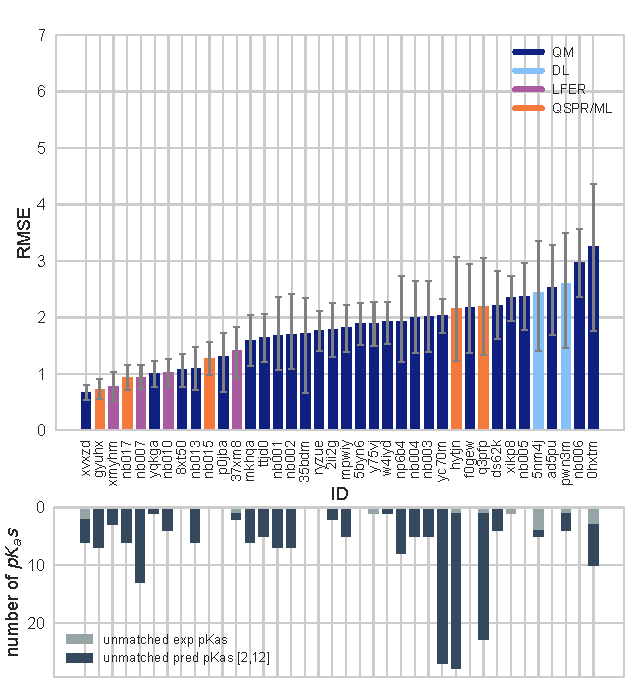
\includegraphics[width=0.5\textwidth]{figures/typeIII-rmse-unmatched-pKa-fig.pdf}}
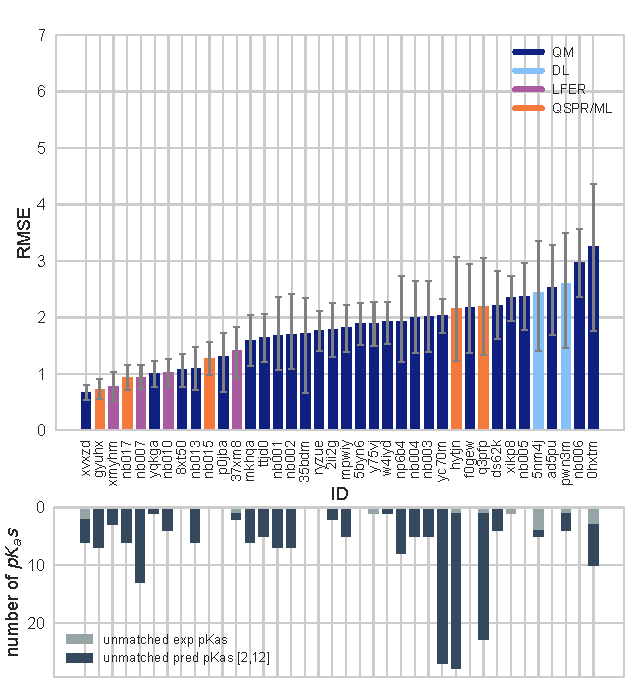
\includegraphics[width=0.5\linewidth]{figures/typeIII-rmse-unmatched-pKa-fig.pdf}
\caption{{\bf RMSE and unmatched \pKa{} counts vs. submission ID plots for macroscopic \pKa{} predictions based on Hungarian matching.} 
Methods are indicated by submission IDs. 
RMSE is shown with error bars denoting 95\% confidence intervals obtained by bootstrapping over challenge molecules. Lower bar plots show the number of unmatched experimental \pKa{}s (light grey, missing predictions) and the number of unmatched \pKa{} predictions (dark grey, extra predictions) for each method between pH 2 and 12. Submission IDs are summarized in Table~\ref{submission-ID-table}. Submission IDs of the form \textit{nb\#\#\#} refer to non-blinded reference methods computed after the blind challenge submission deadline. All others refer to blind, prospective predictions. Submissions are colored by their method categories. Light blue colored database look up methods are utilized as the null prediction method.
}
\label{fig:typeIII-rmse-plot}
\end{figure}



Refer to SI TABLE: Error statistics for all participants.  
Refer to SI FIGURE: Error distribution ridge plots for each method  (exp-pred macroscopic pKa). Which methods tend to overestimate and which methods tend to undestimate?  

\begin{figure}
\centering
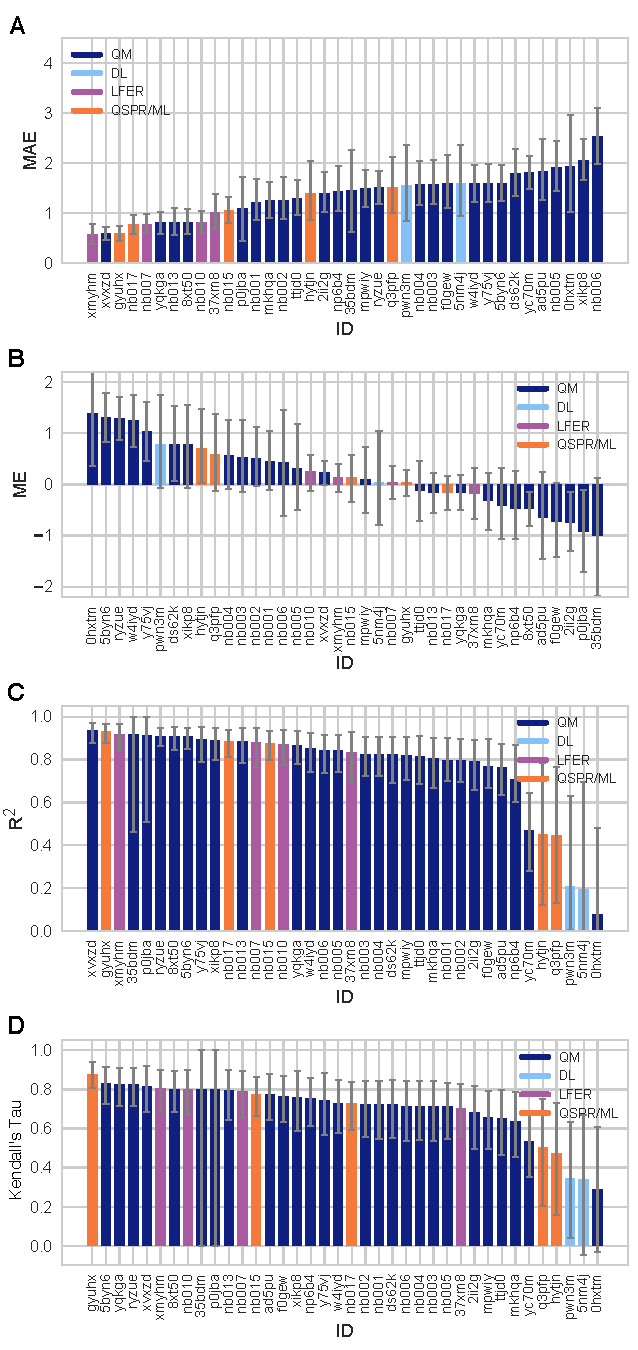
\includegraphics[width=0.5\linewidth]{figures/typeIII_statistics.pdf}
\caption{{\bf Additional performance statistics for macrocopic \pKa{} predictions based on Hungarian matching.} 
Methods are indicated by submission IDs. 
Mean absolute error (MAE), mean error (ME), Pearson’s R\textsuperscript{2}, and Kendall’s Rank Correlation Coefficient Tau ($\tau$) are shown, with error bars denoting 95\% confidence intervals obtained by bootstrapping over challenge molecules. Refer to Table~\ref{submission-ID-table} for submission IDs and method names. Submissions are colored by their method categories. Light blue colored database look up methods are utilized as the null prediction method.
}
\label{fig:typeIII-statistics}
\end{figure}


Describe number of missing and extra pKa for each method.  
Report in total for all molecules how many predicted pKas are there and how many experimental pKas.  
Refer to FIGURE: missing and extra pKa counts.  

Describe overall performance comparison of different methods, grouped by methods class.

\todo[inline]{Explain rationale behind how we analyze the data and determine success/failure}
\todo[inline]{Performance comparison of different methods, grouped by methods class}
Method comparison based on statistical metrics.  
Explain the numerical matching methods used. Explain rationale behind how we analyze the data and determine success/failure.  
Method comparison according to different statistics: RMSE, MAE, ME, R2, m, Kendall's tau.  


\subsubsection{Consistently well performing methods for macroscopic \pKa{} prediction}


\begin{table}[h]
\begin{center}
\begin{threeparttable}
\centering\scriptsize
\caption{{\bf Four consistently well-performing prediction methods for macroscopic \pKa{} prediction based on consistent ranking within the Top~10 according to various statistical metrics.} 
Submissions were ranked according to RMSE, MAE, R\textsuperscript{2}, and $\tau$. Consistently well-performing methods were selected as the ones that rank in the Top~10 in each of these statistical metrics. These methods also have less than 2 unmatched experimental \pKa{}s and less than 7 unmatched predicted \pKa{}s according to Hungarian matching. Performance statistics are provided as mean and 95\% confidence intervals.
} 
\label{well-performing-methods-table}
\begin{tabular}{@{}llllllll@{}}
\toprule
\textbf{Submission ID} & \textbf{Method Name} & \textbf{RMSE} & \textbf{MAE} & \textbf{R\textsuperscript{2}} & \textbf{\begin{tabular}[c]{@{}l@{}}Kendall's Tau \\ ($\tau$)\end{tabular}} & \textbf{\begin{tabular}[c]{@{}l@{}}Unmatched Exp. \\ \pKa{} Count\end{tabular}} & \textbf{\begin{tabular}[c]{@{}l@{}}Unmatched Pred. \\ \pKa{} Count [2,12]\end{tabular}} \\ \midrule
\rowcolor[HTML]{EFEFEF} 
\textit{xvxzd} & \begin{tabular}[c]{@{}l@{}}Full quantum chemical calculation of \\ free energies and fit to experimental pKa\end{tabular} & 0.68 [0.54, 0.81] & 0.58 [0.45, 0.71] & 0.94 [0.88, 0.97] & 0.82 [0.68, 0.92] & 2 & 4 \\
\textit{gyuhx} & S+pKa & 0.73 [0.55, 0.91] & 0.59 [0.44, 0.74] & 0.93 [0.88, 0.96] & 0.88 [0.8, 0.94] & 0 & 7 \\
\rowcolor[HTML]{EFEFEF} 
\textit{xmyhm} & ACD/pKa Classic & 0.79 [0.52, 1.03] & 0.56 [0.38, 0.77] & 0.92 [0.85, 0.97] & 0.81 [0.68, 0.9] & 0 & 3 \\
\textit{8xt50} & \begin{tabular}[c]{@{}l@{}}ReSCoSS conformations // DSD-BLYP-D3 \\ reranking // COSMOtherm pKa\end{tabular} & 1.07 [0.78, 1.36] & 0.81 [0.58, 1.07] & 0.91 [0.84, 0.95] & 0.80 [0.68, 0.89] & 0 & 0 \\ \bottomrule
\end{tabular}
\end{threeparttable}
\end{center}
\end{table}


\todo[inline]{Check if top few performing methods are consistent between error metrics. }


\begin{figure}
\centering
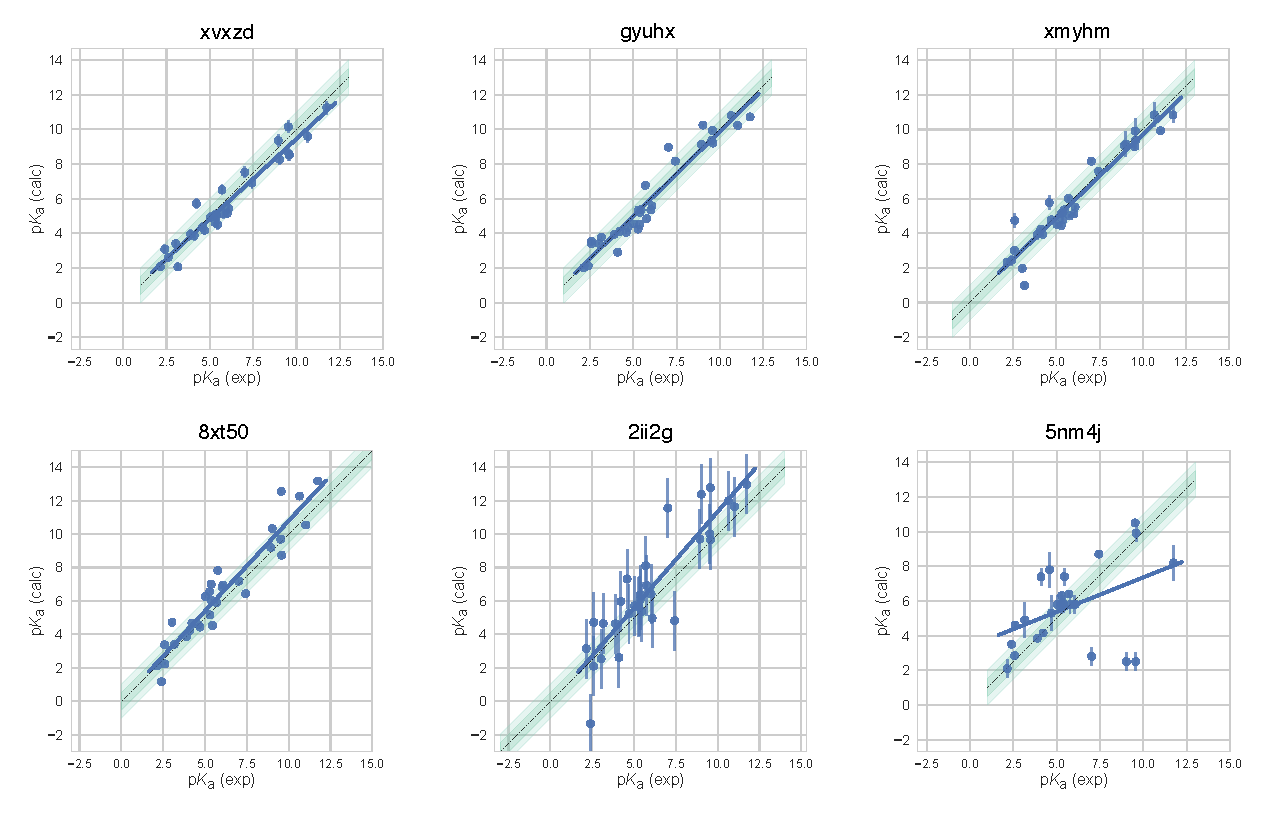
\includegraphics[width=1.0\linewidth]{figures/typeIII-pred-vs-exp-correlation-fig.pdf}
\caption{{\bf Predicted vs. experimental value correlation plots of 4 consistently well-performing methods, a representative method with average performance (\textit{2ii2g}), and the null method (\textit{5nm4j})}. 
Dark and light green shaded areas indicate 0.5 and 1.0 units of error. Error bars indicate standard error of the mean of predicted and experimental values. Experimental \pKa{} SEM values are too small to be seen under the data points. EC-RISM/MP2/cc-pVTZ-P2-q-noThiols-2par method (\textit{2ii2g}) was selected as the representative method with average performance because it is the method with the highest RMSE below the median.
}
\label{fig:typeIII_pred_vs_exp_correlation}
\end{figure}



\subsubsection{Which chemicals are harder to predict?}

For physical prediction methods sulfur containing heterocycles, amide next to aromatic heterocycles, compounds with iodo and bromo domains have lower pKa prediction accuracy.

\begin{figure}
\begin{center}
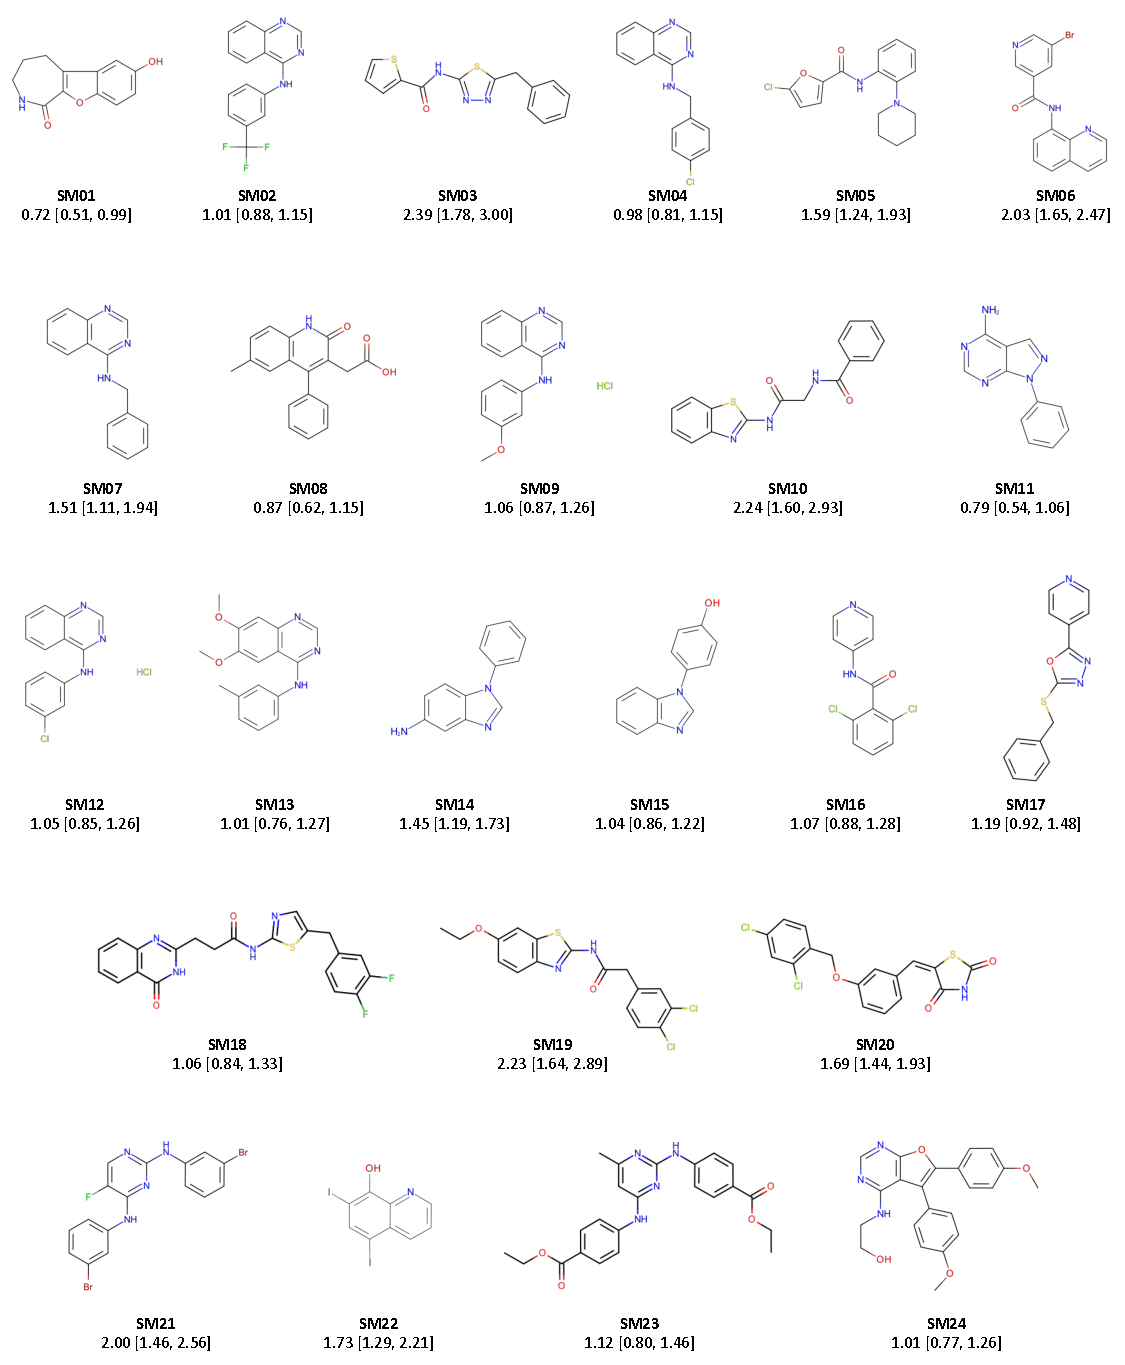
\includegraphics[width=0.95\linewidth]{figures/molecules_with_MAE_of_all_methods.pdf}
\caption{{\bf Molecules of SAMPL6 Challenge with MAE calculated for all macroscopic \pKa{} predictions.} MAE calculated considering all prediction methods indicate which molecules had the lowest prediction accuracy in SAMPL6 Challenge. MAE values calculated for each molecule include all the matched \pKa{} values, which could be more than one per method for multiprotic molecules (SM06, SM14, SM15, SM16, SM18, SM22). Hungarian matching algorithm wasemployed for pairing experimental and predicted \pKa{} values. MAE values are reported with 95\% confidence intervals.
}
\label{fig:molecules_with_MAE_of_all_methods}
\end{center}
\end{figure}

Prediction performance of individual molecules
\todo[inline]{Which chemical structures make pKa predictions more difficult?}
SAMPL6 pKa set consisted of only 24 small molecules which limits our ability to do statistical analysis to determine which chemical substructures contribute to greater errors in pKa predictions.
\todo[inline]{Illustration/explanation of effects where microscopic pKas and macroscopic pKas can differ}

\todo[inline]{Are there any correlations between molecular descriptors and pKa errors?}

\todo[inline]{What can we learn from failures? Which physical effects are driving failures?}








\begin{figure}
\centering
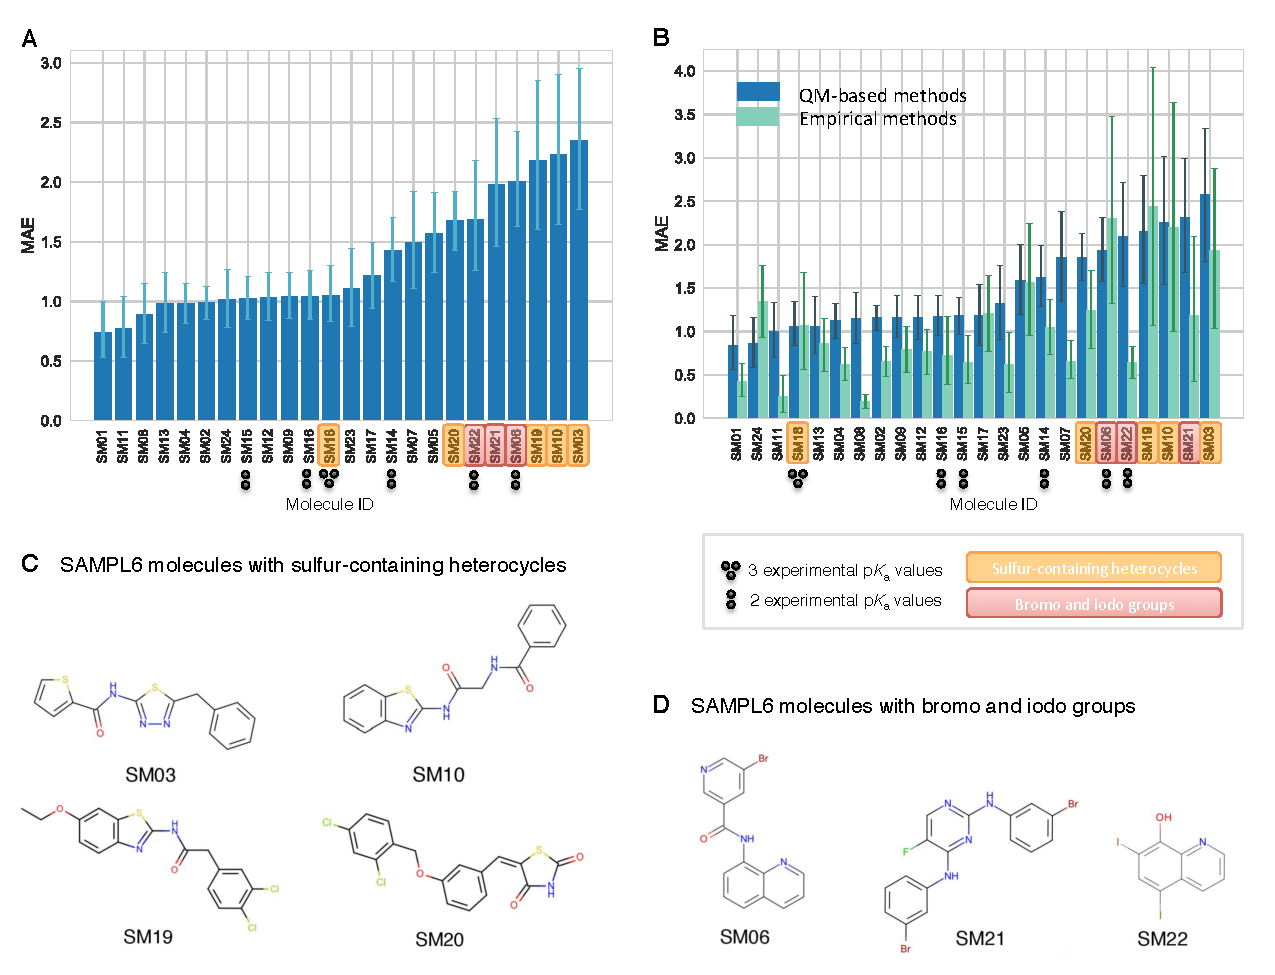
\includegraphics[width=1.0\linewidth]{figures/typeIII_molecular_MAE_fig.pdf}
\caption{{\bf Average prediction accuracy calculated over all prediction methods was lower for molecules with sulfur-containing heterocycles, bromo, and iodo groups.}
{\bf(A)} MAE calculated for each molecule as an average of all methods. {\bf(B)} MAE of each molecule broken out by method category. QM-based methods (blue) include QM predictions with or without linear empirical correction. Empirical methods (green) include QSAR, ML, DL, and LFER approaches. {\bf(C)} Depiction of SAMPL6 molecules with sulfur-containing heterocycles. {\bf(D)} Depiction of SAMPL6 molecules with iodo and bromo groups .
}
\label{fig:typeIII_molecular_MAE}
\end{figure}


\begin{figure}
\centering
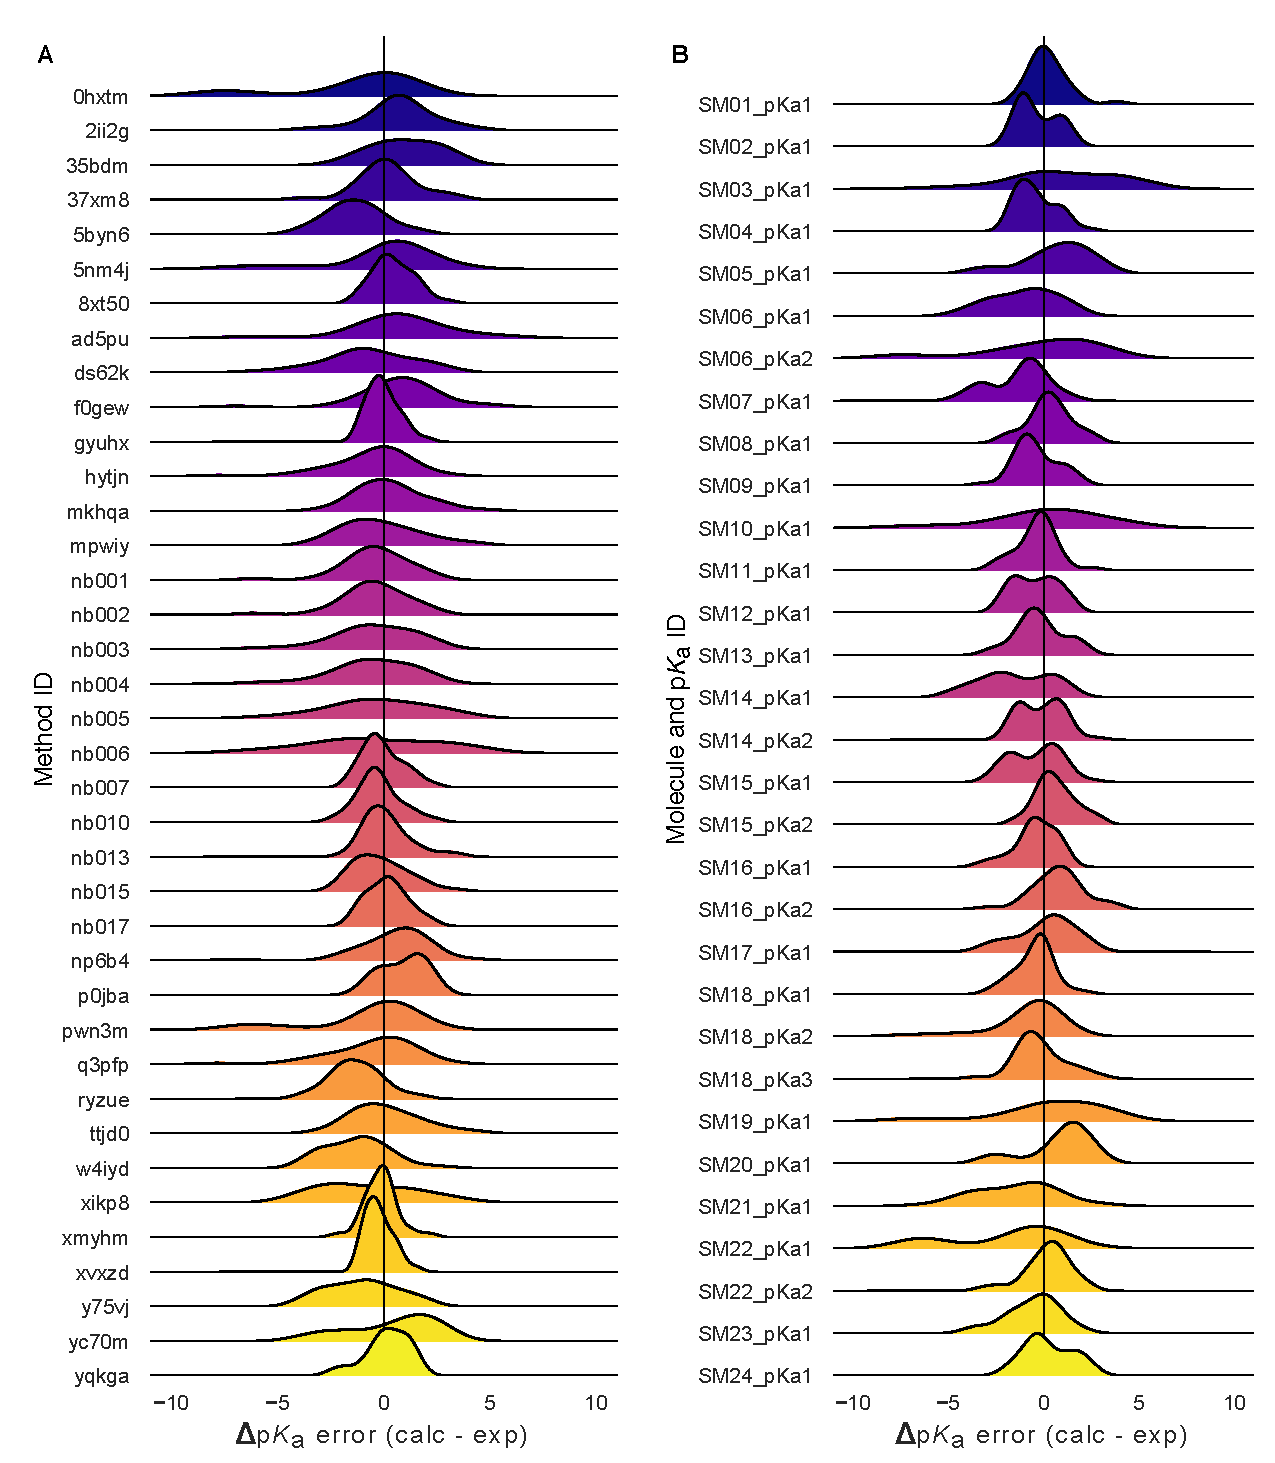
\includegraphics[width=0.8\linewidth]{figures/typeIII-error-distribution.pdf}
\caption{{\bf Macroscopic \pKa{} prediction error distribution plots show how prediction accuracy varies across methods and individual molecules.}
{\bf(A)} \pKa{} prediction error distribution for each submission for all molecules according to Hungarian matching. {\bf(B)} Error distribution for each SAMPL6 molecule for all prediction methods according to Hungarian matching. For multiprotic molecules, \pKa{} ID numbers (pKa1, pKa2, and pKa3) were assigned in the direction of increasing experimental \pKa{} value. 
}
\label{fig:typeIII-error-distribution}
\end{figure}





Does molecular descriptors explain errors/performance ?
We looked for correlation with descriptors, and potential explanation for errors. Keep spurious correlations in mind if we have many descriptors. No correlation observed. Reference the SI Figure of correlations.

\todo[inline]{Comparison of errors/performance against molecular descriptors. Look for correlation with descriptors, and potential explanation for errors. Keep spurious correlations in mind if we have many descriptors.}

Refer to Figure SI: correlation between prediction error and molecular descriptors. There is no clear correlation between molecular descriptors and mean absolute error for each molecule when calculated for all methods.  

Are pKa predictions better in middle region? Error in pKa predictions does not correlate with the true value of pKa.
No correlation between pKa value and error was seen.
Reference the SI Figure.

Refer to Ridge plots of Delta pKa error to identify compounds that were frequently mispredicted.

Compare ME of molecules across methods.
Are there molecules often overestimated or underestimated?

No correlation of macroscopic pKa number to the errors? But we have low representation of multiprotic compounds








%%%
\subsection{Analysis of microscopic \pKa{} predictions using microstates determined by NMR (8 molecules)}




\begin{figure}
\centering
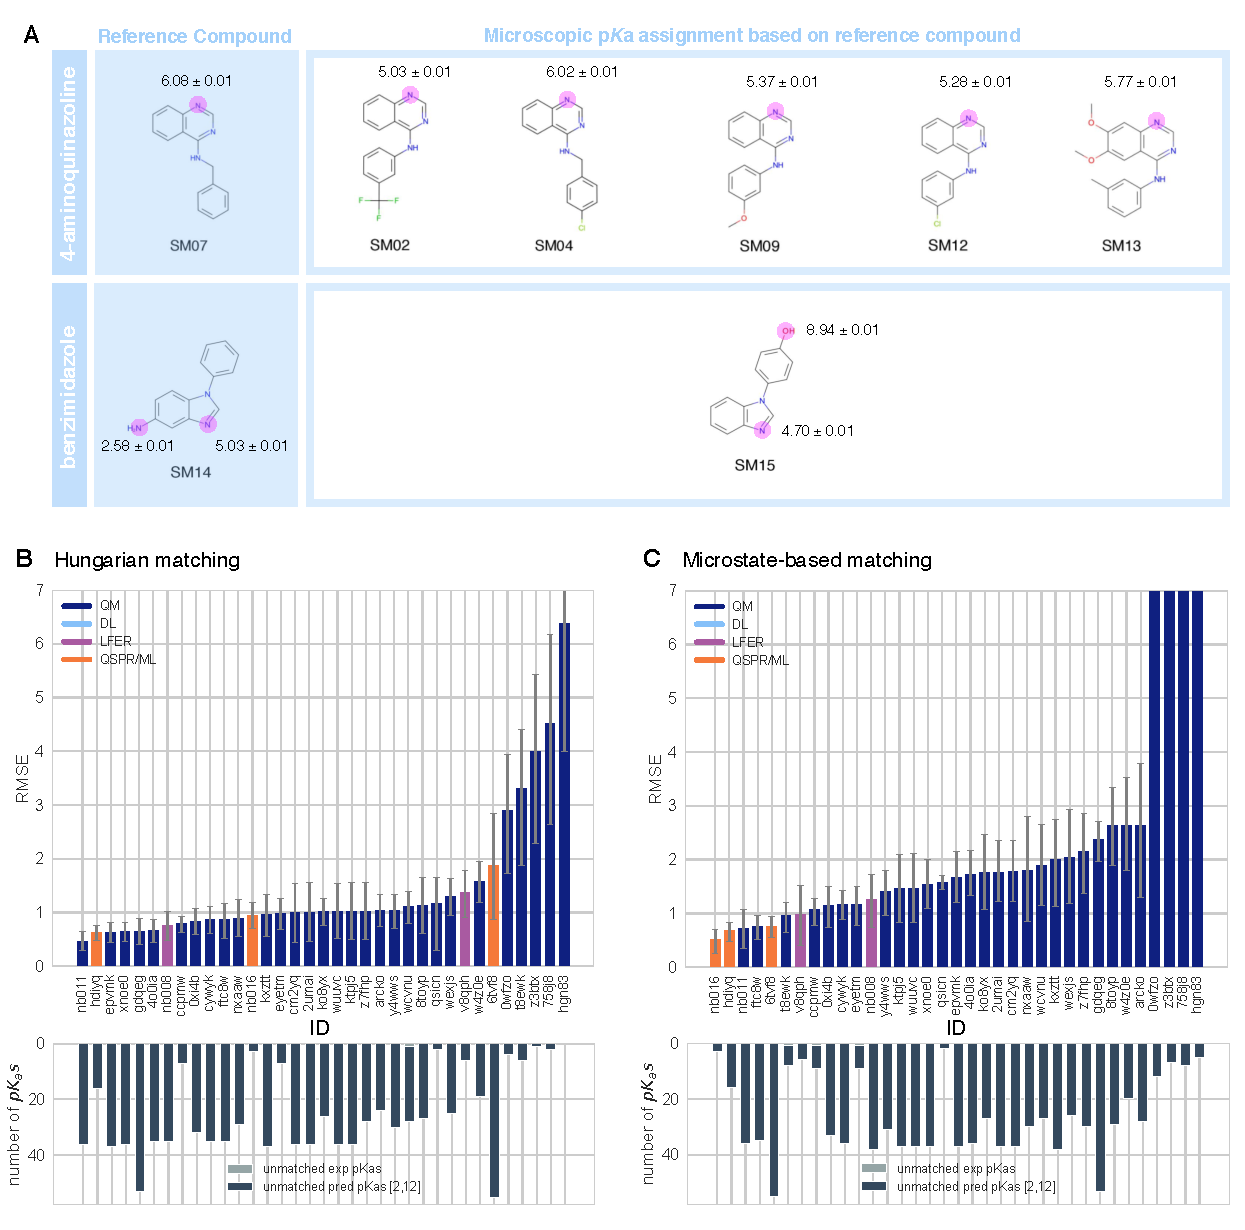
\includegraphics[width=1.0\linewidth]{figures/typeI_8_mol_matching_comparison.pdf}
\caption{{\bf NMR determination of dominant microstates allowed in depth evaluation of microscopic \pKa{} predictions of 8 compounds.} 
{\bf A} Dominant microstate sequence of two compounds (SM07 and SM14) were determined by NMR~\cite{Isik:2018:J.Comput.AidedMol.Des.}. Based on these reference compounds dominant microstates of 6 other derivative compounds were infered and experimental \pKa{} values were assigned to titratable groups with the assumption that only the dominant microstates have significant contributions to the experimentally observed \pKa{}.
{\bf B} RMSE vs. submission ID and unmatched \pKa{} vs. submission ID plots for the evaluation of microscopic \pKa{} predictions of 8 molecules by Hungarian matching to experimental macroscopic \pKa{}s. {\bf C} RMSE vs. submission ID and unmatched \pKa{} vs. submission ID plots showing the evaluation of microscopic \pKa{} predictions of 8 molecules by microstate-based matching between predicted microscopic \pKa{}s and experimental macroscopic \pKa{} values. Submissions \textit{0wfzo, z3btx, 758j8}, and \textit{hgn83} have RMSE values bigger than 10 \pKa{} units which are beyond the y-axis limits of subplot {\bf C} and {\bf B}.
RMSE is shown with error bars denoting 95\% confidence intervals obtained by bootstrapping over challenge molecules. Lower bar plots show the number of unmatched experimental \pKa{}s (light grey, missing predictions) and the number of unmatched \pKa{} predictions (dark grey, extra predictions) for each method between pH 2 and 12. Submission IDs are summarized in Table~\ref{submission-ID-table}. 
}
\label{fig:typeI-matching-algorithm-comparison}
\end{figure}




\subsubsection{Comparing microscopic pKa predictions directly to macroscopic experimental pKa values with numerical matching leads to underestimation of errors}


Demonstrate how numerical matching often masks the error
Match by Hungarian and calculate accuracy of microstate prediction overall.
When matched by pKa value, do people come with the same transition pairs?

Reference Figure~\ref{fig:microstate-pairs-with-Hungarian-match-vs-experiments}  For most methods the microstate pair of Hungarian predicted pKa does not match experimentally determined microstate pair.



Discussion of matching experimental and predicted values
\todo[inline]{Difficulty of assessing predicted pKas using experimental data: matching problem}
\todo[inline]{Explain rationale behind how we analyze the data and determine success/failure}

Compare experimental data to microscopic pKa predictions, assuming experimental pKas are titrations of distinguishable sides and therefore equal to microscopic pKas.
Molecules with only 1 pKa or well separated multiple pKas (more than 3 pKa units apart) SM14 and SM18 were excluded from this analysis, since their experimental pKa values don't satisfy these criteria.

Errors computed by microstate-based matching are larger compared to numerical matching algorithms.
Microscopic pKa analysis with numerical matching algorithms may mask errors due to higher number of guesses made.




Conclusions will only be about 4-aminoquinazoline series and benzimidazole (8 molecules, 10 pKas)
Refer to SI figure of dominant microstates.

Choosing molecules with right protonation state is important.
Do people predict the correct sequence of dominant microstates?
 " Even if your pKa prediction is correct, protonation state prediction can be wrong."
 Analyze which state has lowest free energy for each charge group ( The sequence of "experimentally visible states")



\subsubsection{Accuracy of predicted pKa values when microstate matching is used}

\todo[inline]{Assessment of individual methods by each of our analysis methods}
\todo[inline]{Performance comparison of different methods, grouped by methods class}

\todo[inline]{Comment on the ranking of microscopic pKa prediction error statistsics for all participants (8 mol, microstate match). Refer to Fig.~\ref{fig:typeI-statistics}}

\begin{figure}
\centering
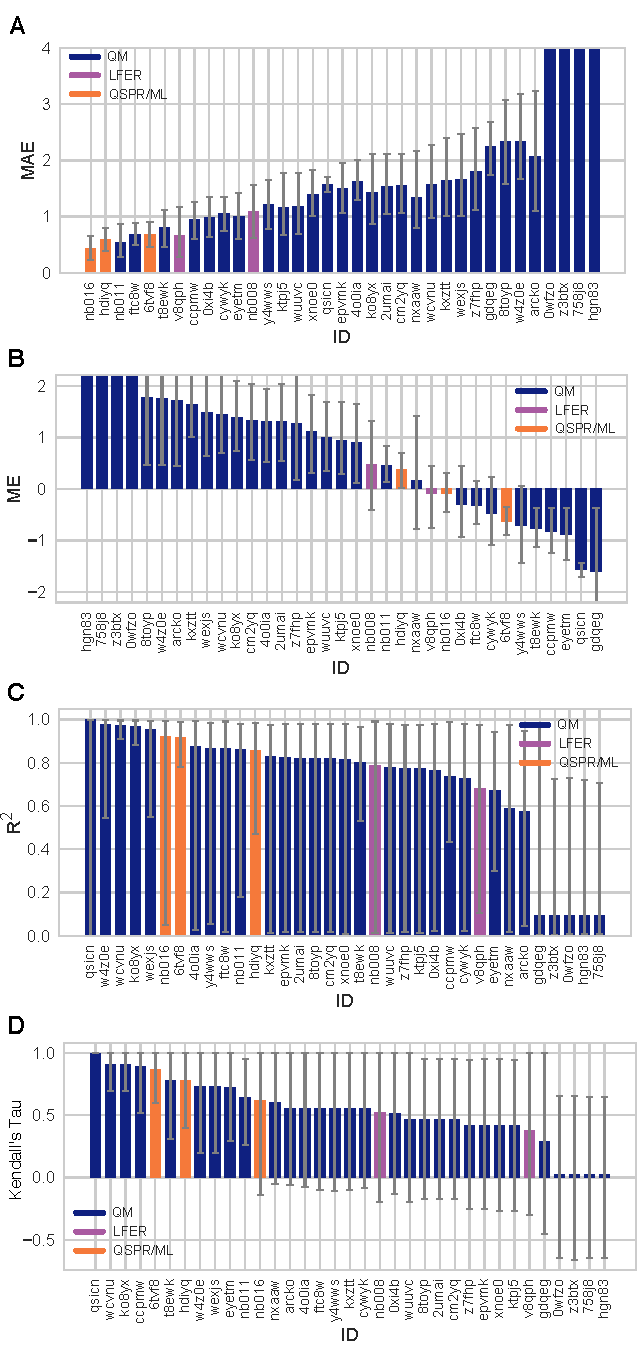
\includegraphics[width=0.5\linewidth]{figures/typeI_statistics.pdf}
\caption{{\bf Additional performance statistics for microscopic \pKa{} predictions for 8 molecules with experimentally determined dominant microstates.} 
Microstate-based matching was performed between experimental \pKa{} values and predicted microscopic \pKa{}s. 
Mean absolute error (MAE), mean error (ME), Pearson’s R\textsuperscript{2}, and Kendall’s Rank Correlation Coefficient Tau ($\tau$) are shown, with error bars denoting 95\% confidence intervals obtained by bootstrapping over challenge molecules. Methods are indicated by submission IDs. Submissions are colored by their method categories. Refer to Table~\ref{submission-ID-table} for submission IDs and method names. Submissions \textit{0wfzo, z3btx, 758j8}, and \textit{hgn83} have MAE and ME values bigger than 10 \pKa{} units which are beyond the y-axis limits of subplots {\bf A} and {\bf B}. A large number and wide variety of methods have a statistically indistinguishable performance based on correlation based statistic ({\bf C} and {\bf D}), in part because of the relatively small dynamic range the small size of the set of 8 molecules.
}
\label{fig:typeI-statistics}
\end{figure}






\subsubsection{Dominant microstate prediction accuracy of methods}

Calculate relative free energy of microstates to determine dominant microstate of each charge
Compare predicted and experimental dominant microstates and calculate accuracy of each method



\begin{figure}
\centering
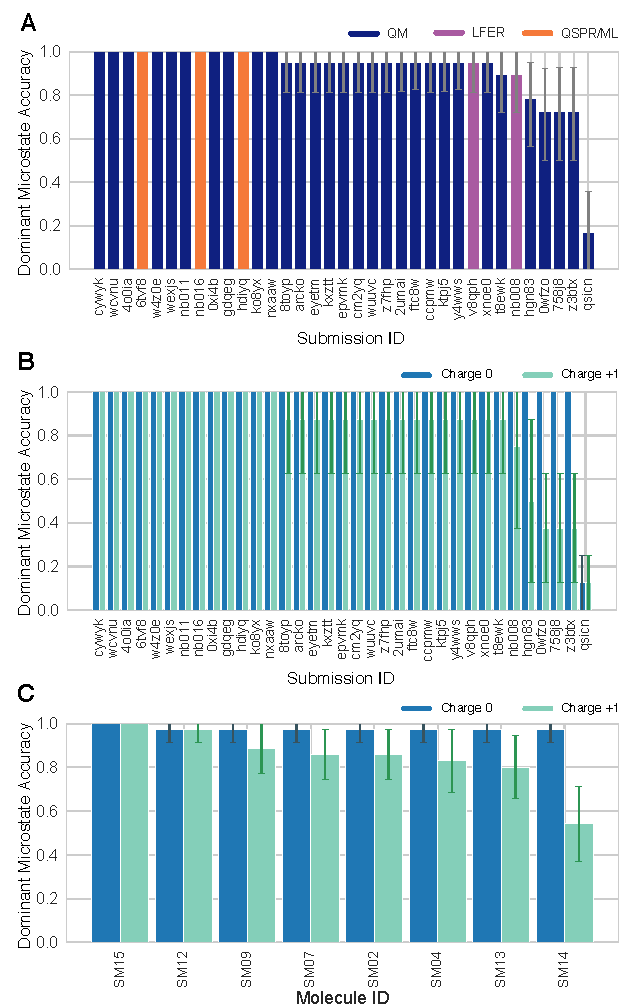
\includegraphics[width=0.5\linewidth]{figures/typeI_dominant_microstate_accuracy.pdf}
\caption{{\bf Some methods predicted the sequence of dominant tautomers inaccurately.} Prediction accuracy of dominant microstate of each charged state was calculated using the dominant microstate sequence determined by NMR for 8 molecules as reference. 
{\bf(A)} Dominant microstate accuracy vs. submission ID plot was calculated considering all the dominant microstates seen in the 8 molecule experimental microstate dataset. {\bf(B)} Dominant microstate accuracy vs. submission ID plot was generating considering only the dominant microstates of charge 0 and +1 seen in the 8 molecule experimental microstate dataset. Accuracy of each molecule is broken out by total charge of the microstate. {\bf(C)} Dominant microstate prediction accuracy calculated for each molecule averaged over all methods. In {\bf(B)} and {\bf(C)}, the accuracy of predicting the dominant neutral tautomer is showed in blue and the accuracy of predicting the dominant +1 charged tautomer is showed in green. Error bars denoting 95\% confidence intervals obtained by bootstrapping.
}
\label{fig:typeI_dominant_microstate_accuracy}
\end{figure}


What percent of the time predictions capture the dominant protonation state correctly? 
Match by microstate and calculate RMSE and MAE. If you know the microstates, can you predict the value of the pKa right? 


\todo[inline]{Does top 3 methods predict the same dominant microstate sequence? How differently do different methods predict microscopic transitions? (method vs method correlation plot to see if methods predict the same microstate pairs or not)}


\subsubsection{Which molecules caused lower dominant microstate prediction accuracy?}

Which molecule has more errors in predicting the major microstates?



\todo[inline]{Comment on consensus prediction accuracy. Comparison of predicted microstates using consensus set of transitions of high accuracy prediction methods} 






%%% 
\subsection{Analyzing microscopic pKa prediction from the perspective of thermodynamics}
Explain  linearity  relative free energy of protonation states with respect to pH. Free energy perspective simplifies data capturing and analysis. Reference Marilyn's paper.

Thermodynamic cycle closure checking allows evaluation of microsopic pKas  without experimental data.
Checking for thermodynamic consistency


\subsubsection{Cycle closure error}
\todo[inline]{
- Introduce linear protonation state free energy diagram [Cite Gunner et al 2019 paper]  
FIGURE: linear plot of free energy vs pH  
}

Marilyn observed very good cycle closure results and very bad one that are up to 10 kcal/mol
 
She suggesting checking the cycle with maximum cycle closure error for each method and reporting that for each method.
An historgam of max cycle closure error will help us bin these results into 3 categoris:
1. good agreement
2. moderate
3. severe 
 
"We think thermodyamic cycles of protonation states need to be closed"
Message: Methods need to checked for cycle closure errors.
There can be information there that can be used to correct pKa predictions.
When cycles are not closed it may be used as an indicator of prediction uncertainty.

%%%
\subsection{How would pKa errors affect protein-ligand binding affinity predictions?}
\todo[inline]{Illustrate the ways in which the pKa errors can influence prediction errors for binding affinities}
\todo[inline]{How do accuracy limitations in small molecule pKa prediction translate into modeling errors in ligand affinity prediction?}
In addition, determining the free energy penalty of such states~\citep{deOliveira:2019:J.Chem.TheoryComput.} also requires knowing the \pKa{} value. 

\todo[inline]{EQUATION: free energy of protonation state equation}


$$ \Delta G_{bind} =\Delta G_{bind}^{C} + \Delta G_{prot}$$  

$$ \Delta G_{bind} =\Delta G_{bind}^{C} + RT(pH - pK_a) \ln{(10)}$$

$$ \Delta G_{bind} =\Delta G_{bind}^{N} + \Delta G_{corr}$$  

$$ \Delta G_{bind} =\Delta G_{bind}^{N} - RT\ln{\frac{1 + e^{-\frac{\Delta G_{bind}^{C} - \Delta G_{bind}^{N}}{RT}}10^{pK_a - pH}}{1 + 10^{pK_a - pH}}} $$  


\begin{figure}
\centering
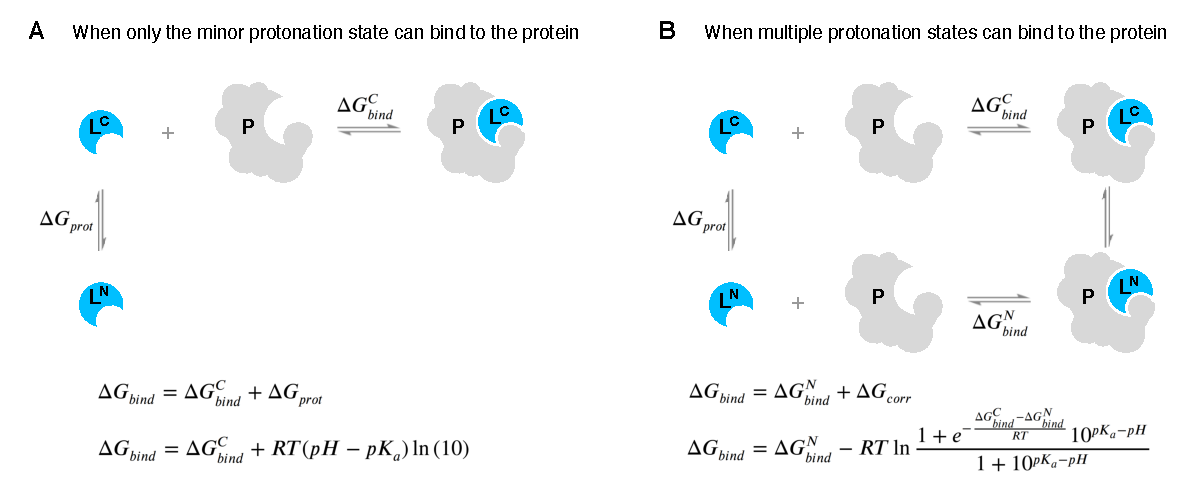
\includegraphics[width=1.0\linewidth]{figures/pKa-effects-on-protein-ligand-binding.pdf}
\caption{ {\bf Aqueous \pKa{} of the ligand can influence overall protein-ligand binding affinity.} {\bf A} When only the minor aqueous protonation state contributes to protein-ligand complex formation, overall binding free energy ($\Delta G_{bind}$) needs to be calculated as the sum of binding affinity of the minor state and the protonation penalty of that state. {\bf B} When multiple charge states contribute to complex formation, overall free energy of binding includes a multiple protonation states correction (MPSC) term ($\Delta G_{corr}$). MPSC is a function of pH, aqueous \pKa{} of the ligand, and the difference between the binding free energy of charged and neutral species ($\Delta G_{bind}^{C} - \Delta G_{bind}^{N}$).
}
\label{fig:pKa-effects-on-protein-ligand-binding}
\end{figure}

\begin{figure}
\centering
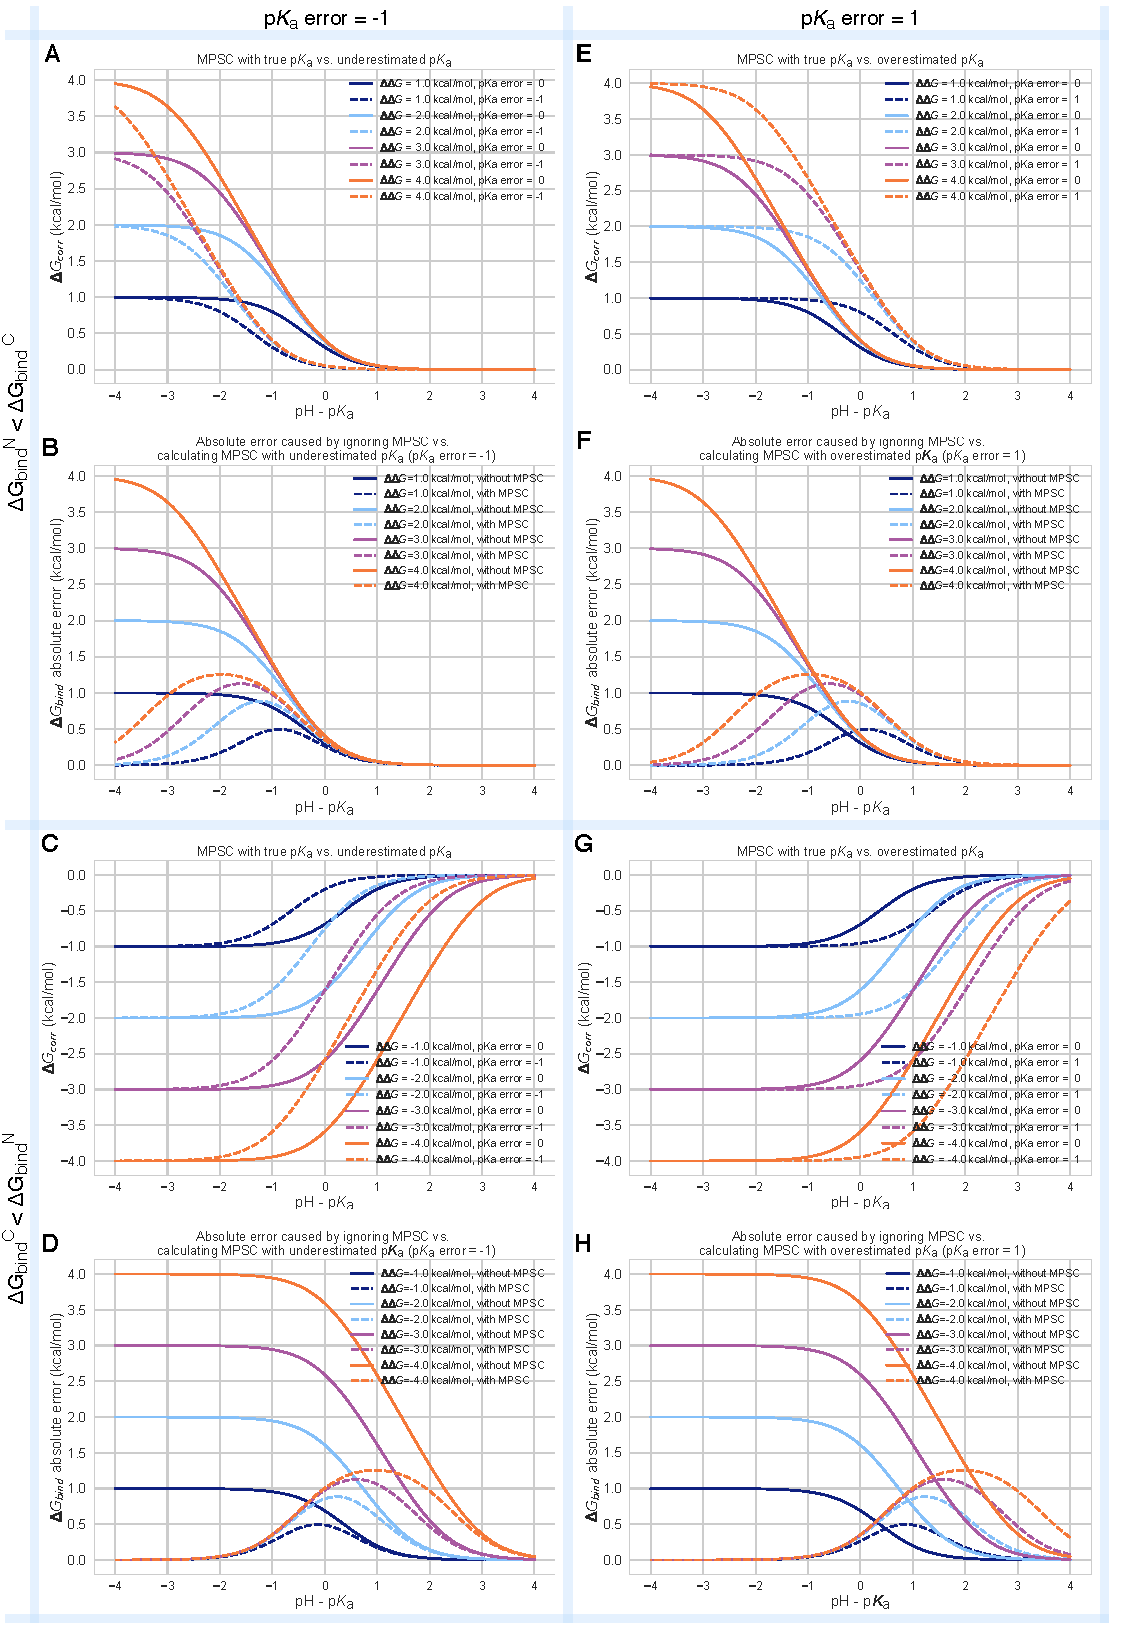
\includegraphics[width=0.8\linewidth]{figures/pKa-inaccuracy-and-MPSC.pdf}
\caption{ {\bf Inaccuracy of \pKa{} prediction ($\pm$ 1 unit) affects the the accuracy of MPSC and overall protein-ligand binding free energy calculation in varying amounts based on aqueous \pKa{} value and relative binding affinity of individual protonation states ($\Delta\Delta G = \Delta G_{bind}^{C} - \Delta G_{bind}^{N}$).} 
All calculations are made for 25\degree C, and for a ligand with single basic titratable group. {\bf A, C, E, and G} show MPSC ($\Delta G_{corr}$) calculated with true vs. inaccurate \pKa{}. {\bf B, D, F, and H} show comparison of the absolute error to $\Delta G_{bind}$ caused by ignoring the MPSC completely (solid lines) vs. calculating MPSC based in inaccurate \pKa{} value (dashed lines). These plots provide guidence on when it is beneficial to include MPSC correction based on \pKa{} error, pH - \pKa{}, and $\Delta\Delta G$. 
}
\label{fig:pKa-inaccuracy-and-MPSC}
\end{figure}



%%%
\subsection{Lessons learned from SAMPL6 pKa Challenge}
\todo[inline]{Do any methods predict within experimental accuracy (how is the field doing overall)?}
\todo[inline]{Common challenging factors for accurate pKa predictions. Tautomers, Heterocycles etc.}

Overall results:  
Do any methods predict within experimental accuracy (how is the field doing overall)?
Common challenging factors for accurate pKa predictions. Tautomers, Heterocycles etc.

Discussion of matching problem betwene experimental and predicted values.  
Difficulty of assessing predicted pKas using experimental data: matching problem
Explain rationale behind how we analyze the data and determine success/failure.

Conclusion about prediction performance of individual molecules:
SAMPL6 pKa set consisted of only 24 small molecules which limits our ability to do statistical analysis to determine which chemical substructures contribute to greater errors in pKa predictions.  
Which chemical structures make pKa predictions more difficult?  

What can we learn from failures? Which physical effects are driving failures?
Cycle closure errors


%%%
\subsection{Suggestions for future challenges}
In the SAMPL6 \pKa{} Challenge there wasn't a requirement that prediction sets should report predictions for all compounds. 
Some participants reported predictions for only a subset of compounds which may lead these methods to look more accurate than others, due to missing predictions.
It would have been a better choice to require submissions for whole sets for better comparison of method performance. 

\todo[inline]{Discuss what can be done to further improve future challenges}
How can we maximize what we learn?
What should we have people predict?
How should we select compounds / measure pKas?

\todo[inline]{Suggestions about challenge construction}
Future challenge direction  
Challenge path: predict pKas, give people pKas to predict logDs on same molecules, then predict for new set of compounds logDs without provided pKas.  

Enumeration of protonation states before predictions (which states does one need to consider?)

\todo[inline]{Suggestions about challenge analysis}

NMR experimental techniques could be used to validate microstate information in future challenges

Reporting microscopic pKa predictions with charges, microstate free energies is betetr
Experimental dataset with microstate infromation is more helpful.

What can be done to further improve future challenges
How can we maximize what we learn?
What should we have people predict?
How should we select compounds / measure pKas? NMR experimental techniques could be used to validate microstate information in future challenges

Suggestions about challenge construction
Enumeration of protonation states before predictions (which states does one need to consider?)
Suggestions about challenge analysis


%%%%%%%%%%%%%%%%%%%%%%%%%%%%%%%%%%%%%%%%%%%%%%%%%%%%%%%%%%%%














%%%%%%%%%%%%%%%%%%%%%%%%%%%%%%%%%%%%%%%%%%%%%%%%%%%%%%%%%%%%
% Conclusion
%%%%%%%%%%%%%%%%%%%%%%%%%%%%%%%%%%%%%%%%%%%%%%%%%%%%%%%%%%%%
\section{Conclusion}


%%%%%%%%%%%%%%%%%%%%%%%%%%%%%%%%%%%%%%%%%%%%%%%%%%%%%%%%%%%%
% Code and Data Availability
%%%%%%%%%%%%%%%%%%%%%%%%%%%%%%%%%%%%%%%%%%%%%%%%%%%%%%%%%%%%
\section{Code and data availability}
\begin{minipage}{15cm}
\begin{itemize}

\item SAMPL6 \pKa{} challenge instructions, submissions, experimental data and analysis is available at  \href{https://github.com/samplchallenges/SAMPL6}{https://github.com/samplchallenges/SAMPL6}

\end{itemize}
\end{minipage}


%%%%%%%%%%%%%%%%%%%%%%%%%%%%%%%%%%%%%%%%%%%%%%%%%%%%%%%%%%%%
% Overview of supplementary information
%%%%%%%%%%%%%%%%%%%%%%%%%%%%%%%%%%%%%%%%%%%%%%%%%%%%%%%%%%%%
\section{Overview of supplementary information}

\paragraph{Contents of the Supplementary Information:}

\begin{itemize}
\item TABLE~\ref{pKa_chemical_identifiers_table}: SMILES and InChI identifiers of SAMPL6 \pKa{}  Challenge molecules.
\item TABLE~\ref{SI_statistics_table_macro_pKa}: Evaluation statistics calculated for all macroscopic \pKa{} prediction submissions based on Hungarian match for 24 molecules.
\item TABLE~\ref{SI-statistics-table-micro-pKa-8mol-hungarian}: Evaluation statistics calculated for all microscopic \pKa{} prediction submissions based on Hungarian match for 8 molecules with NMR data.
\item TABLE~\ref{SI-statistics-table-micro-pKa-8mol-microstate}: Evaluation statistics calculated for all microscopic \pKa{} prediction submissions based on microstate match for 8 molecules with NMR data.
\item FIGURE~\ref{fig:experimental-microstate-IDs-SI-table}: Dominant microstates of 8 molecules were determined based on NMR measurements.
\item FIGURE~\ref{fig:molecular_properties_vs_MAE_correlation}: MAE of macroscopic \pKa{} predictions of each molecule did not show any significant correlation with any molecular descriptor.
\item FIGURE~\ref{fig:macroscopic-pKa-error-vs-pKa-value}: The value of macroscopic \pKa{} was not a factor affecting prediction error seen in SAMPL6 Challenge according to the analysis with Hungarian matching.
\item FIGURE~\ref{fig:microstate-pairs-with-Hungarian-match-vs-experiments}: There was low agreement between experimental dominant microstate pairs and the predicted microstate pairs selected by Hungarian algorithm for microscopic \pKa{} predictions. 




\end{itemize}

\paragraph{Extra files included in \textit{SAMPL6-supplementary-documents.tar.gz}:}  
\begin{itemize}
\item SAMPL6-pKa-chemical-identifiers-table.csv 
\item macroscopic-pKa-statistics-24mol-hungarian-match.csv
\item microscopic-pKa-statistics-8mol-hungarian-match-table.csv
\item microscopic-pKa-statistics-8mol-microstate-match-table.csv
\item experimental-microstates-of-8mol-based-on-NMR.csv
\item enumerate-microstates-with-Epik-and-OpenEye-Quakpac.ipynb
\item molecule\_ID\_and\_SMILES.csv
\end{itemize}


%%%%%%%%%%%%%%%%%%%%%%%%%%%%%%%%%%%%%%%%%%%%%%%%%%%%%%%%%%%%
% Author Contributions 
%%%%%%%%%%%%%%%%%%%%%%%%%%%%%%%%%%%%%%%%%%%%%%%%%%%%%%%%%%%%
\section{Author Contributions}

Conceptualization, MI, JDC, CB, DLM ; Methodology, MI, JDC ; Software, MI, AR, ASR ; Formal Analysis, MI, ASR, AR ; Investigation, MI ; Resources, JDC;  Data Curation, MI ; Writing-Original Draft, MI, JDC; Writing - Review and Editing, MI, ASR, AR, CB, DLM, JDC; Visualization, MI, AR ; Supervision, JDC, DLM, CB, ASR ; Project Administration, MI ; Funding Acquisition, JDC, DLM.

%(Follow the \href{http://www.cell.com/pb/assets/raw/shared/guidelines/CRediT-taxonomy.pdf}{CRediT Taxonomy})

%%%%%%%%%%%%%%%%%%%%%%%%%%%%%%%%%%%%%%%%%%%%%%%%%%%%%%%%%%%%
% Acknowledgments 
%%%%%%%%%%%%%%%%%%%%%%%%%%%%%%%%%%%%%%%%%%%%%%%%%%%%%%%%%%%%
\section{Acknowledgments}

\todo[inline]{Complete acknowledgments section. Caitlin Bannan, Thomas Fox}
MI, ASR, and JDC acknowledge support from the Sloan Kettering Institute.
JDC acknowledges support from NIH grant P30 CA008748. 
MI acknowledges Doris J.\ Hutchinson Fellowship. 
We thank Brad Sherborne for his valuable insights at the conception of the \pKa{} challenge and connecting us with Timothy Rhodes and Dorothy Levorse who were able to provide resources and expertise for experimental measurements performed at MRL. 
We acknowledge Paul Czodrowski who provided feedback on multiple stages of this work: challenge construction, purchasable compound selection and manuscript. 
MI, ASR, AR and JDC are grateful to OpenEye Scientific for providing a free academic software license for use in this work.

Mike Chui
%\todo[inline]{JDC: Can we cite the ORCIDs of people we thank in this work?}

%%%%%%%%%%%%%%%%%%%%%%%%%%%%%%%%%%%%%%%%%%%%%%%%%%%%%%%%%%%%
% Disclosures 
%%%%%%%%%%%%%%%%%%%%%%%%%%%%%%%%%%%%%%%%%%%%%%%%%%%%%%%%%%%%
\section{Disclosures}

JDC is a member of the Scientific Advisory Board for Schr\"{o}dinger, LLC.
DLM is a member of the Scientific Advisory Board of OpenEye Scientific Software.

Table ref: \cite{ACD-pKa-galas, ACD-pKa-classic, simulation-plus-pKa, chemicalize-pKa, moka-pKa}
trial: [], +, -, *, \#, \textbackslash{}m

%%%%%%%%%%%%%%%%%%%%%%%%%%%%%%%%%%%%%%%%%%%%%%%%%%%%%%%%%%%%
%%% BIBLIOGRAPHY
%%%%%%%%%%%%%%%%%%%%%%%%%%%%%%%%%%%%%%%%%%%%%%%%%%%%%%%%%%%%


%\nocite{*} % This command displays all refs in the bib file. PLEASE DELETE IT BEFORE YOU SUBMIT YOUR MANUSCRIPT!
\bibliography{zotero, manual}


%%%%%%%%%%%%%%%%%%%%%%%%%%%%%%%%%%%%%%%%%%%%%%%%%%%%%%%%%%%%
% Supplementary Information
%%%%%%%%%%%%%%%%%%%%%%%%%%%%%%%%%%%%%%%%%%%%%%%%%%%%%%%%%%%%
\newpage
\beginsupplement
\section{Supplementary Information}











\begin{table}[tb!]
\begin{center}
\begin{threeparttable}
\centering\scriptsize
\caption{{\bf SMILES and InChI identifiers of SAMPL6 \pKa{}  Challenge molecules.} A CSV version of this table can be found in \textit{SAMPL6-supplementary-documents.tar.gz}.
} 
\centering\scriptsize
\label{pKa_chemical_identifiers_table}
\begin{tabular}{@{}lll@{}}
\toprule
SAMPL6 Molecule ID & Isomeric SMILES & InChI \\ \midrule
\rowcolor[HTML]{EFEFEF} 
SM01 & c1cc2c(cc1O)c3c(o2)C(=O)NCCC3 & \begin{tabular}[c]{@{}l@{}}InChI=1S/C12H11NO3/c14-7-3-4-10-9(6-7)8-2-1-5-13-12(15)11(8)16-10/\\ h3-4,6,14H,1-2,5H2,(H,13,15)\end{tabular} \\
SM02 & c1ccc2c(c1)c(ncn2)Nc3cccc(c3)C(F)(F)F & \begin{tabular}[c]{@{}l@{}}InChI=1S/C15H10F3N3/c16-15(17,18)10-4-3-5-11(8-10)21-14-12-6-1-2-7\\ -13(12)19-9-20-14/h1-9H,(H,19,20,21)\end{tabular} \\
\rowcolor[HTML]{EFEFEF} 
SM03 & c1ccc(cc1)Cc2nnc(s2)NC(=O)c3cccs3 & \begin{tabular}[c]{@{}l@{}}InChI=1S/C14H11N3OS2/c18-13(11-7-4-8-19-11)15-14-17-16-12(20-14)9\\ -10-5-2-1-3-6-10/h1-8H,9H2,(H,15,17,18)\end{tabular} \\
SM04 & c1ccc2c(c1)c(ncn2)NCc3ccc(cc3)Cl & \begin{tabular}[c]{@{}l@{}}InChI=1S/C15H12ClN3/c16-12-7-5-11(6-8-12)9-17-15-13-3-1-2-4-14(13)1\\ 8-10-19-15/h1-8,10H,9H2,(H,17,18,19)\end{tabular} \\
\rowcolor[HTML]{EFEFEF} 
SM05 & c1ccc(c(c1)NC(=O)c2ccc(o2)Cl)N3CCCCC3 & \begin{tabular}[c]{@{}l@{}}InChI=1S/C16H17ClN2O2/c17-15-9-8-14(21-15)16(20)18-12-6-2-3-7-13(1\\ 2)19-10-4-1-5-11-19/h2-3,6-9H,1,4-5,10-11H2,(H,18,20)\end{tabular} \\
SM06 & c1cc2cccnc2c(c1)NC(=O)c3cc(cnc3)Br & \begin{tabular}[c]{@{}l@{}}InChI=1S/C15H10BrN3O/c16-12-7-11(8-17-9-12)15(20)19-13-5-1-3-10-4-2\\ -6-18-14(10)13/h1-9H,(H,19,20)\end{tabular} \\
\rowcolor[HTML]{EFEFEF} 
SM07 & c1ccc(cc1)CNc2c3ccccc3ncn2 & \begin{tabular}[c]{@{}l@{}}InChI=1S/C15H13N3/c1-2-6-12(7-3-1)10-16-15-13-8-4-5-9-14(13)17-11-18\\ -15/h1-9,11H,10H2,(H,16,17,18)\end{tabular} \\
SM08 & Cc1ccc2c(c1)c(c(c(=O)[nH]2)CC(=O)O)c3ccccc3 & \begin{tabular}[c]{@{}l@{}}InChI=1S/C18H15NO3/c1-11-7-8-15-13(9-11)17(12-5-3-2-4-6-12)14(10-16\\ (20)21)18(22)19-15/h2-9H,10H2,1H3,(H,19,22)(H,20,21)\end{tabular} \\
\rowcolor[HTML]{EFEFEF} 
SM09 & COc1cccc(c1)Nc2c3ccccc3ncn2.Cl & \begin{tabular}[c]{@{}l@{}}InChI=1S/C15H13N3O.ClH/c1-19-12-6-4-5-11(9-12)18-15-13-7-2-3-8-14(1\\ 3)16-10-17-15;/h2-10H,1H3,(H,16,17,18);1H\end{tabular} \\
SM10 & c1ccc(cc1)C(=O)NCC(=O)Nc2nc3ccccc3s2 & \begin{tabular}[c]{@{}l@{}}InChI=1S/C16H13N3O2S/c20-14(10-17-15(21)11-6-2-1-3-7-11)19-16-18-1\\ 2-8-4-5-9-13(12)22-16/h1-9H,10H2,(H,17,21)(H,18,19,20)\end{tabular} \\
\rowcolor[HTML]{EFEFEF} 
SM11 & c1ccc(cc1)n2c3c(cn2)c(ncn3)N & \begin{tabular}[c]{@{}l@{}}InChI=1S/C11H9N5/c12-10-9-6-15-16(11(9)14-7-13-10)8-4-2-1-3-5-8/h1-7\\ H,(H2,12,13,14)\end{tabular} \\
SM12 & c1ccc2c(c1)c(ncn2)Nc3cccc(c3)Cl.Cl & \begin{tabular}[c]{@{}l@{}}InChI=1S/C14H10ClN3.ClH/c15-10-4-3-5-11(8-10)18-14-12-6-1-2-7-13(12)\\ 16-9-17-14;/h1-9H,(H,16,17,18);1H\end{tabular} \\
\rowcolor[HTML]{EFEFEF} 
SM13 & Cc1cccc(c1)Nc2c3cc(c(cc3ncn2)OC)OC & \begin{tabular}[c]{@{}l@{}}InChI=1S/C17H17N3O2/c1-11-5-4-6-12(7-11)20-17-13-8-15(21-2)16(22-3)9\\ -14(13)18-10-19-17/h4-10H,1-3H3,(H,18,19,20)\end{tabular} \\
SM14 & c1ccc(cc1)n2cnc3c2ccc(c3)N & \begin{tabular}[c]{@{}l@{}}InChI=1S/C13H11N3/c14-10-6-7-13-12(8-10)15-9-16(13)11-4-2-1-3-5-11/h1\\ -9H,14H2\end{tabular} \\
\rowcolor[HTML]{EFEFEF} 
SM15 & c1ccc2c(c1)ncn2c3ccc(cc3)O & \begin{tabular}[c]{@{}l@{}}InChI=1S/C13H10N2O/c16-11-7-5-10(6-8-11)15-9-14-12-3-1-2-4-13(12)15/\\ h1-9,16H\end{tabular} \\
SM16 & c1cc(c(c(c1)Cl)C(=O)Nc2ccncc2)Cl & \begin{tabular}[c]{@{}l@{}}InChI=1S/C12H8Cl2N2O/c13-9-2-1-3-10(14)11(9)12(17)16-8-4-6-15-7-5-8/\\ h1-7H,(H,15,16,17)\end{tabular} \\
\rowcolor[HTML]{EFEFEF} 
SM17 & c1ccc(cc1)CSc2nnc(o2)c3ccncc3 & \begin{tabular}[c]{@{}l@{}}InChI=1S/C14H11N3OS/c1-2-4-11(5-3-1)10-19-14-17-16-13(18-14)12-6-8-\\ 15-9-7-12/h1-9H,10H2\end{tabular} \\
SM18 & c1ccc2c(c1)c(=O)[nH]c(n2)CCC(=O)Nc3ncc(s3)Cc4ccc(c(c4)F)F & \begin{tabular}[c]{@{}l@{}}InChI=1S/C21H16F2N4O2S/c22-15-6-5-12(10-16(15)23)9-13-11-24-21(30\\ -13)27-19(28)8-7-18-25-17-4-2-1-3-14(17)20(29)26-18/h1-6,10-11H,7-9H2,\\ (H,24,27,28)(H,25,26,29)\end{tabular} \\
\rowcolor[HTML]{EFEFEF} 
SM19 & CCOc1ccc2c(c1)sc(n2)NC(=O)Cc3ccc(c(c3)Cl)Cl & \begin{tabular}[c]{@{}l@{}}InChI=1S/C17H14Cl2N2O2S/c1-2-23-11-4-6-14-15(9-11)24-17(20-14)21-1\\ 6(22)8-10-3-5-12(18)13(19)7-10/h3-7,9H,2,8H2,1H3,(H,20,21,22)\end{tabular} \\
SM20 & c1cc(cc(c1)OCc2ccc(cc2Cl)Cl)/C=C/3\textbackslash{}C(=O)NC(=O)S3 & \begin{tabular}[c]{@{}l@{}}InChI=1S/C17H11Cl2NO3S/c18-12-5-4-11(14(19)8-12)9-23-13-3-1-2-10(6-\\ 13)7-15-16(21)20-17(22)24-15/h1-8H,9H2,(H,20,21,22)/b15-7+\end{tabular} \\
\rowcolor[HTML]{EFEFEF} 
SM21 & c1cc(cc(c1)Br)Nc2c(cnc(n2)Nc3cccc(c3)Br)F & \begin{tabular}[c]{@{}l@{}}InChI=1S/C16H11Br2FN4/c17-10-3-1-5-12(7-10)21-15-14(19)9-20-16(23-\\ 15)22-13-6-2-4-11(18)8-13/h1-9H,(H2,20,21,22,23)\end{tabular} \\
SM22 & c1cc2c(cc(c(c2nc1)O)I)I & InChI=1S/C9H5I2NO/c10-6-4-7(11)9(13)8-5(6)2-1-3-12-8/h1-4,13H \\
\rowcolor[HTML]{EFEFEF} 
SM23 & CCOC(=O)c1ccc(cc1)Nc2cc(nc(n2)Nc3ccc(cc3)C(=O)OCC)C & \begin{tabular}[c]{@{}l@{}}InChI=1S/C23H24N4O4/c1-4-30-21(28)16-6-10-18(11-7-16)25-20-14-15(3)\\ 24-23(27-20)26-19-12-8-17(9-13-19)22(29)31-5-2/h6-14H,4-5H2,1-3H3,(H2,\\ 24,25,26,27)\end{tabular} \\
SM24 & COc1ccc(cc1)c2c3c(ncnc3oc2c4ccc(cc4)OC)NCCO & \begin{tabular}[c]{@{}l@{}}InChI=1S/C22H21N3O4/c1-27-16-7-3-14(4-8-16)18-19-21(23-11-12-26)24-\\ 13-25-22(19)29-20(18)15-5-9-17(28-2)10-6-15/h3-10,13,26H,11-12H2,1-2H3,\\ (H,23,24,25)\end{tabular} \\ \bottomrule
\end{tabular}
\end{threeparttable}
\end{center}
\end{table}



\begin{table}[tb!]
\begin{center}
\begin{threeparttable}
\centering\scriptsize
\caption{{\bf Evaluation statistics calculated for all macroscopic \pKa{} prediction submissions based on Hungarian match for 24 molecules.} Methods are represented via their SAMPL6 submission IDs which can be cross referenced with Table~\ref{submission-ID-table} for method details. There are eight error metrics reported: the root-mean-squared error (RMSE), mean absolute error (MAE), mean (signed) error (ME), coefficient of determination (R\textsuperscript{2}), linear regression slope (m), Kendall’s Rank Correlation Coefficient ($\tau$), unmatched experimental \pKa{}s (number of missing \pKa{} predictions) and unmatched predicted \pKa{}s (number of extra \pKa{} predictions between 2 and 12. This table is ranked by increasing RMSE. A CSV version of this table can be found in \textit{SAMPL6-supplementary-documents.tar.gz}. } 
\centering\scriptsize
\label{SI_statistics_table_macro_pKa}
\begin{tabular}{@{}lllllllll@{}}
\toprule
\textbf{\begin{tabular}[c]{@{}l@{}}Submission \\ ID\end{tabular}} & \textbf{RMSE} & \textbf{MAE} & \textbf{ME} & \textbf{R\textsuperscript{2}} & \textbf{m} & \textbf{Kendall's Tau} & \textbf{\begin{tabular}[c]{@{}l@{}}Unmatched \\ exp. \pKa{}s\end{tabular}} & \textbf{\begin{tabular}[c]{@{}l@{}}Unmatched \\ pred. \pKa{}s [2,12]\end{tabular}} \\ \midrule
\textit{xvxzd} & 0.68 [0.54, 0.81] & 0.58 [0.45, 0.71] & 0.24 [-0.01, 0.45] & 0.94 [0.88, 0.97] & 0.92 [0.84, 1.02] & 0.82 [0.68, 0.92] & 2 & 4 \\
\textit{gyuhx} & 0.73 [0.55, 0.91] & 0.59 [0.44, 0.74] & 0.03 [-0.23, 0.28] & 0.93 [0.88, 0.96] & 0.98 [0.90, 1.08] & 0.88 [0.80, 0.94] & 0 & 7 \\
\textit{xmyhm} & 0.79 [0.52, 1.03] & 0.56 [0.38, 0.77] & 0.13 [-0.14, 0.41] & 0.92 [0.85, 0.97] & 0.96 [0.86, 1.08] & 0.81 [0.68, 0.90] & 0 & 3 \\
\textit{nb017} & 0.94 [0.72, 1.16] & 0.77 [0.58, 0.97] & -0.16 [-0.49, 0.16] & 0.88 [0.81, 0.94] & 0.94 [0.82, 1.08] & 0.73 [0.60, 0.84] & 0 & 6 \\
\textit{nb007} & 0.95 [0.73, 1.15] & 0.78 [0.60, 0.97] & 0.05 [-0.29, 0.37] & 0.88 [0.77, 0.95] & 0.84 [0.77, 0.92] & 0.79 [0.65, 0.89] & 0 & 13 \\
\textit{yqkga} & 1.01 [0.78, 1.23] & 0.80 [0.59, 1.03] & -0.17 [-0.51, 0.19] & 0.87 [0.78, 0.93] & 0.93 [0.77, 1.08] & 0.83 [0.72, 0.91] & 0 & 1 \\
\textit{nb010} & 1.03 [0.77, 1.26] & 0.81 [0.61, 1.04] & 0.24 [-0.11, 0.59] & 0.87 [0.77, 0.94] & 0.95 [0.83, 1.08] & 0.80 [0.67, 0.90] & 0 & 4 \\
\textit{8xt50} & 1.07 [0.78, 1.36] & 0.81 [0.58, 1.07] & -0.47 [-0.82, -0.14] & 0.91 [0.84, 0.95] & 1.08 [0.94, 1.22] & 0.80 [0.68, 0.89] & 0 & 0 \\
\textit{nb013} & 1.10 [0.72, 1.47] & 0.80 [0.56, 1.09] & -0.15 [-0.55, 0.22] & 0.88 [0.78, 0.95] & 1.09 [0.90, 1.25] & 0.79 [0.64, 0.90] & 0 & 6 \\
\textit{nb015} & 1.27 [0.98, 1.56] & 1.04 [0.80, 1.31] & 0.13 [-0.32, 0.56] & 0.87 [0.80, 0.93] & 1.16 [0.94, 1.34] & 0.78 [0.66, 0.86] & 0 & 0 \\
\textit{p0jba} & 1.31 [0.69, 1.73] & 1.08 [0.43, 1.72] & -0.92 [-1.72, -0.11] & 0.91 [0.51, 1.00] & 1.18 [0.36, 1.72] & 0.80 [0.00, 1.00] & 0 & 0 \\
\textit{37xm8} & 1.41 [0.93, 1.84] & 1.01 [0.68, 1.38] & -0.18 [-0.69, 0.32] & 0.83 [0.70, 0.93] & 1.16 [0.98, 1.33] & 0.70 [0.56, 0.83] & 1 & 1 \\
\textit{mkhqa} & 1.60 [1.13, 2.05] & 1.24 [0.90, 1.62] & -0.32 [-0.89, 0.21] & 0.80 [0.67, 0.91] & 1.14 [0.98, 1.34] & 0.64 [0.44, 0.79] & 0 & 6 \\
\textit{ttjd0} & 1.64 [1.20, 2.06] & 1.30 [0.96, 1.67] & -0.12 [-0.70, 0.45] & 0.81 [0.69, 0.91] & 1.2 [1.03, 1.40] & 0.65 [0.47, 0.80] & 0 & 5 \\
\textit{nb001} & 1.68 [1.05, 2.37] & 1.21 [0.84, 1.68] & 0.44 [-0.10, 1.03] & 0.80 [0.70, 0.90] & 1.16 [0.95, 1.42] & 0.72 [0.55, 0.85] & 0 & 7 \\
\textit{nb002} & 1.70 [1.08, 2.38] & 1.25 [0.89, 1.70] & 0.51 [-0.04, 1.10] & 0.80 [0.70, 0.90] & 1.15 [0.95, 1.42] & 0.72 [0.56, 0.84] & 0 & 7 \\
\textit{35bdm} & 1.72 [0.66, 2.34] & 1.44 [0.62, 2.26] & -1.01 [-2.18, 0.13] & 0.92 [0.46, 1.00] & 1.45 [0.73, 2.15] & 0.80 [0.00, 1.00] & 0 & 0 \\
\textit{ryzue} & 1.77 [1.42, 2.12] & 1.50 [1.17, 1.84] & 1.30 [0.86, 1.72] & 0.91 [0.86, 0.95] & 1.23 [1.06, 1.41] & 0.82 [0.71, 0.91] & 0 & 0 \\
\textit{2ii2g} & 1.80 [1.31, 2.24] & 1.39 [1.01, 1.82] & -0.74 [-1.29, -0.15] & 0.79 [0.65, 0.89] & 1.15 [0.96, 1.37] & 0.68 [0.59, 0.82] & 0 & 2 \\
\textit{mpwiy} & 1.82 [1.39, 2.23] & 1.48 [1.14, 1.88] & 0.10 [-0.54, 0.73] & 0.82 [0.70, 0.91] & 1.29 [1.12, 1.51] & 0.66 [0.49, 0.80] & 0 & 5 \\
\textit{5byn6} & 1.89 [1.50, 2.27] & 1.59 [1.24, 1.97] & 1.32 [0.84, 1.80] & 0.91 [0.85, 0.95] & 1.28 [1.10, 1.48] & 0.83 [0.72, 0.92] & 0 & 0 \\
\textit{y75vj} & 1.90 [1.50, 2.26] & 1.58 [1.21, 1.97] & 1.04 [0.46, 1.60] & 0.89 [0.79, 0.95] & 1.34 [1.16, 1.53] & 0.75 [0.57, 0.88] & 1 & 0 \\
\textit{w4iyd} & 1.93 [1.53, 2.28] & 1.58 [1.20, 1.98] & 1.26 [0.72, 1.76] & 0.85 [0.74, 0.92] & 1.21 [1.00, 1.4.0] & 0.73 [0.57, 0.85] & 0 & 1 \\
\textit{np6b4} & 1.94 [1.21, 2.71] & 1.44 [1.04, 1.94] & -0.47 [-1.08, 0.24] & 0.71 [0.60, 0.87] & 1.08 [0.81, 1.43] & 0.75 [0.62, 0.86] & 0 & 8 \\
\textit{nb004} & 2.01 [1.38, 2.63] & 1.57 [1.16, 2.04] & 0.56 [-0.10, 1.27] & 0.82 [0.72, 0.90] & 1.35 [1.15, 1.60] & 0.71 [0.54, 0.84] & 0 & 5 \\
\textit{nb003} & 2.01 [1.39, 2.64] & 1.58 [1.18, 2.04] & 0.52 [-0.14, 1.22] & 0.82 [0.73, 0.91] & 1.36 [1.16, 1.61] & 0.71 [0.54, 0.84] & 0 & 5 \\
\textit{yc70m} & 2.03 [1.73, 2.33] & 1.80 [1.48, 2.13] & -0.41 [-1.09, 0.31] & 0.47 [0.28, 0.64] & 0.56 [0.35, 0.83] & 0.53 [0.35, 0.68] & 0 & 27 \\
\textit{hytjn} & 2.16 [1.24, 3.06] & 1.39 [0.86, 2.04] & 0.71 [0.03, 1.48] & 0.45 [0.13, 0.78] & 0.62 [0.26, 1.00] & 0.47 [0.16, 0.73] & 1 & 27 \\
\textit{f0gew} & 2.18 [1.38, 2.95] & 1.58 [1.09, 2.16] & -0.73 [-1.42, 0.04] & 0.77 [0.67, 0.89] & 1.29 [1.01, 1.63] & 0.76 [0.63, 0.86] & 0 & 0 \\
\textit{q3pfp} & 2.19 [1.33, 3.09] & 1.51 [0.99, 2.13] & 0.59 [-0.10, 1.37] & 0.44 [0.13, 0.77] & 0.66 [0.27, 1.07] & 0.50 [0.20, 0.75] & 1 & 22 \\
\textit{ds62k} & 2.22 [1.62, 2.81] & 1.78 [1.34, 2.27] & 0.78 [0.06, 1.52] & 0.82 [0.70, 0.90] & 1.41 [1.20, 1.63] & 0.72 [0.55, 0.85] & 0 & 4 \\
\textit{xikp8} & 2.35 [1.94, 2.73] & 2.06 [1.66, 2.47] & 0.77 [-0.02, 1.58] & 0.89 [0.80, 0.95] & 1.59 [1.40, 1.81] & 0.76 [0.59, 0.89] & 1 & 0 \\
\textit{nb005} & 2.38 [1.79, 2.95] & 1.91 [1.44, 2.43] & 0.31 [-0.49, 1.15] & 0.84 [0.74, 0.91] & 1.56 [1.34, 1.82] & 0.71 [0.54, 0.83] & 0 & 0 \\
\textit{5nm4j} & 2.45 [1.42, 3.34] & 1.58 [0.94, 2.34] & 0.05 [-0.80, 1.07] & 0.19 [0.00, 0.70] & 0.40 [-0.06, 0.81] & 0.34 [-0.04, 0.67] & 4 & 1 \\
\textit{ad5pu} & 2.54 [1.68, 3.30] & 1.83 [1.24, 2.49] & -0.65 [-1.48, 0.25] & 0.76 [0.64, 0.88] & 1.43 [1.12, 1.78] & 0.77 [0.63, 0.88] & 0 & 0 \\
\textit{pwn3m} & 2.60 [1.45, 3.53] & 1.54 [0.83, 2.37] & 0.79 [-0.06, 1.77] & 0.21 [0.00, 0.63] & 0.37 [0.01, 0.78] & 0.34 [0.04, 0.63] & 1 & 3 \\
\textit{nb006} & 2.98 [2.37, 3.56] & 2.53 [2.00, 3.10] & 0.42 [-0.60, 1.47] & 0.84 [0.74, 0.92] & 1.78 [1.55, 2.06] & 0.71 [0.54, 0.84] & 0 & 0 \\
\textit{0hxtm} & 3.26 [1.81, 4.39] & 1.92 [1.03, 2.98] & 1.38 [0.37, 2.56] & 0.08 [0.00, 0.48] & 0.28 [-0.17, 0.83] & 0.29 [-0.04, 0.61] & 3 & 7 \\ \bottomrule
\end{tabular}
\end{threeparttable}
\end{center}
\end{table}



\begin{table}[tb!]
\begin{center}
\begin{threeparttable}
\centering\scriptsize
\caption{{\bf Evaluation statistics calculated for all microscopic \pKa{} prediction submissions based on Hungarian match for 8 molecules with NMR data.} Methods are represented via their SAMPL6 submission IDs which can be cross referenced with Table~\ref{submission-ID-table} for method details. There are eight error metrics reported: the root-mean-squared error (RMSE), mean absolute error (MAE), mean (signed) error (ME), coefficient of determination (R\textsuperscript{2}), linear regression slope (m), Kendall’s Rank Correlation Coefficient ($\tau$), unmatched experimental \pKa{}s (number of missing \pKa{} predictions) and unmatched predicted \pKa{}s (number of extra \pKa{} predictions between 2 and 12. This table is ranked by increasing RMSE. A CSV version of this table can be found in \textit{SAMPL6-supplementary-documents.tar.gz}. } 
\centering\scriptsize
\label{SI-statistics-table-micro-pKa-8mol-hungarian}
\begin{tabular}{@{}lllllllll@{}}
\toprule
\textbf{\begin{tabular}[c]{@{}l@{}}Submission \\ ID\end{tabular}} & \textbf{RMSE} & \textbf{MAE} & \textbf{ME} & \textbf{R\textsuperscript{2}} & \textbf{m} & \textbf{Kendall's Tau} & \textbf{\begin{tabular}[c]{@{}l@{}}Unmatched \\ exp. \pKa{}s\end{tabular}} & \textbf{\begin{tabular}[c]{@{}l@{}}Unmatched \\ pred. \pKa{}s [2,12]\end{tabular}} \\ \midrule
\textit{nb011} & 0.47 [0.30, 0.64] & 0.33 [0.22, 0.46] & -0.02 [-0.18, 0.14] & 0.97 [0.94, 0.99] & 1.01 [0.97, 1.06] & 0.90 [0.78, 0.96] & 0 & 36 \\
\textit{hdiyq} & 0.62 [0.47, 0.76] & 0.47 [0.33, 0.62] & 0.13 [-0.09, 0.34] & 0.95 [0.92, 0.97] & 0.34 [0.92, 1.09] & 0.87 [0.79, 0.93] & 0 & 16 \\
\textit{epvmk} & 0.63 [0.43, 0.81] & 0.47 [0.32, 0.63] & -0.02 [-0.25, 0.21] & 0.95 [0.89, 0.98] & 0.21 [0.91, 1.04] & 0.81 [0.68, 0.91] & 0 & 37 \\
\textit{xnoe0} & 0.65 [0.47, 0.82] & 0.50 [0.36, 0.66] & -0.1 [-0.32, 0.13] & 0.95 [0.89, 0.98] & 0.13 [0.92, 1.05] & 0.82 [0.69, 0.91] & 0 & 36 \\
\textit{gdqeg} & 0.65 [0.41, 0.89] & 0.43 [0.27, 0.62] & 0.11 [-0.10, 0.35] & 0.94 [0.88, 0.98] & 0.35 [0.87, 1.02] & 0.83 [0.67, 0.95] & 0 & 53 \\
\textit{4o0ia} & 0.66 [0.44, 0.86] & 0.47 [0.31, 0.64] & 0.00 [-0.22, 0.24] & 0.94 [0.88, 0.98] & 0.24 [0.87, 1.05] & 0.85 [0.73, 0.94] & 0 & 35 \\
\textit{nb008} & 0.76 [0.48, 1.02] & 0.52 [0.34, 0.73] & -0.08 [-0.37, 0.17] & 0.93 [0.85, 0.98] & 0.17 [0.79, 0.93] & 0.84 [0.73, 0.92] & 0 & 35 \\
\textit{ccpmw} & 0.79 [0.62, 0.94] & 0.62 [0.46, 0.80] & -0.17 [-0.44, 0.11] & 0.92 [0.86, 0.96] & 0.11 [0.82, 1.05] & 0.80 [0.67, 0.89] & 0 & 7 \\
\textit{0xi4b} & 0.84 [0.58, 1.07] & 0.61 [0.42, 0.83] & 0.22 [-0.07, 0.51] & 0.92 [0.84, 0.97] & 0.51 [0.91, 1.09] & 0.81 [0.65, 0.92] & 0 & 32 \\
\textit{cywyk} & 0.86 [0.60, 1.10] & 0.62 [0.42, 0.84] & 0.13 [-0.16, 0.44] & 0.90 [0.82, 0.96] & 0.44 [0.86, 1.08] & 0.81 [0.64, 0.92] & 0 & 35 \\
\textit{ftc8w} & 0.86 [0.51, 1.17] & 0.59 [0.39, 0.83] & 0.10 [-0.19, 0.41] & 0.90 [0.77, 0.97] & 0.41 [0.84, 0.98] & 0.75 [0.57, 0.88] & 0 & 35 \\
\textit{nxaaw} & 0.89 [0.56, 1.25] & 0.61 [0.41, 0.87] & -0.02 [-0.35, 0.28] & 0.89 [0.75, 0.97] & 0.28 [0.85, 1.00] & 0.79 [0.63, 0.91] & 0 & 29 \\
\textit{nb016} & 0.95 [0.71, 1.18] & 0.77 [0.57, 0.98] & -0.23 [-0.56, 0.12] & 0.89 [0.83, 0.95] & 0.12 [0.82, 1.07] & 0.75 [0.62, 0.85] & 0 & 3 \\
\textit{kxztt} & 0.96 [0.56, 1.33] & 0.64 [0.41, 0.92] & 0.00 [-0.32, 0.36] & 0.90 [0.76, 0.97] & 0.36 [0.96, 1.13] & 0.79 [0.63, 0.91] & 0 & 37 \\
\textit{eyetm} & 0.98 [0.69, 1.27] & 0.72 [0.50, 0.97] & -0.32 [-0.65, 0.00] & 0.91 [0.86, 0.96] & 0.00 [0.94, 1.22] & 0.78 [0.64, 0.88] & 0 & 7 \\
\textit{cm2yq} & 0.99 [0.44, 1.54] & 0.56 [0.31, 0.90] & 0.10 [-0.21, 0.50] & 0.91 [0.83, 0.98] & 0.50 [0.96, 1.25] & 0.89 [0.80, 0.96] & 0 & 36 \\
\textit{2umai} & 1.00 [0.46, 1.54] & 0.57 [0.33, 0.91] & 0.07 [-0.25, 0.46] & 0.91 [0.82, 0.98] & 0.46 [0.96, 1.26] & 0.87 [0.76, 0.95] & 0 & 36 \\
\textit{ko8yx} & 1.01 [0.76, 1.25] & 0.78 [0.56, 1.01] & 0.35 [0.01, 0.67] & 0.91 [0.82, 0.96] & 0.67 [0.96, 1.19] & 0.78 [0.64, 0.89] & 0 & 26 \\
\textit{wuuvc} & 1.02 [0.51, 1.53] & 0.62 [0.38, 0.93] & 0.19 [-0.13, 0.58] & 0.88 [0.80, 0.96] & 0.58 [0.85, 1.19] & 0.90 [0.81, 0.96] & 0 & 36 \\
\textit{ktpj5} & 1.02 [0.51, 1.56] & 0.61 [0.37, 0.95] & 0.17 [-0.16, 0.57] & 0.88 [0.80, 0.96] & 0.57 [0.87, 1.22] & 0.89 [0.80, 0.96] & 0 & 36 \\
\textit{z7fhp} & 1.02 [0.49, 1.55] & 0.61 [0.36, 0.94] & 0.08 [-0.24, 0.48] & 0.90 [0.82, 0.97] & 0.48 [0.97, 1.26] & 0.88 [0.80, 0.95] & 0 & 28 \\
\textit{arcko} & 1.04 [0.73, 1.32] & 0.77 [0.53, 1.02] & 0.37 [0.05, 0.72] & 0.89 [0.80, 0.94] & 0.72 [0.90, 1.14] & 0.78 [0.62, 0.90] & 0 & 24 \\
\textit{y4wws} & 1.04 [0.70, 1.33] & 0.74 [0.49, 1.00] & -0.31 [-0.66, 0.05] & 0.91 [0.85, 0.96] & 0.05 [1.02, 1.26] & 0.79 [0.68, 0.88] & 0 & 30 \\
\textit{wcvnu} & 1.11 [0.80, 1.39] & 0.84 [0.59, 1.11] & 0.28 [-0.10, 0.66] & 0.89 [0.77, 0.95] & 0.66 [0.98, 1.22] & 0.73 [0.54, 0.88] & 1 & 27 \\
\textit{8toyp} & 1.13 [0.61, 1.65] & 0.70 [0.42, 1.05] & 0.13 [-0.25, 0.56] & 0.88 [0.81, 0.96] & 0.56 [0.98, 1.29] & 0.83 [0.72, 0.92] & 0 & 27 \\
\textit{qsicn} & 1.17 [0.30, 1.65] & 0.88 [0.23, 1.54] & -0.76 [-1.54, 0.01] & 0.91 [0.46, 1.00] & 0.01 [0.52, 1.59] & 0.80 [0.00, 1.00] & 0 & 2 \\
\textit{wexjs} & 1.30 [0.95, 1.62] & 0.98 [0.68, 1.29] & 0.27 [-0.17, 0.74] & 0.86 [0.74, 0.93] & 0.74 [1.00, 1.29] & 0.73 [0.55, 0.86] & 0 & 25 \\
\textit{v8qph} & 1.37 [0.92, 1.79] & 0.98 [0.66, 1.34] & -0.15 [-0.64, 0.34] & 0.84 [0.70, 0.93] & 0.34 [0.97, 1.32] & 0.70 [0.55, 0.82] & 0 & 6 \\
\textit{w4z0e} & 1.57 [1.18, 1.94] & 1.23 [0.90, 1.58] & 0.09 [-0.48, 0.62] & 0.85 [0.76, 0.91] & 0.62 [1.08, 1.46] & 0.72 [0.60, 0.82] & 0 & 19 \\
\textit{6tvf8} & 1.88 [0.87, 2.85] & 1.02 [0.54, 1.66] & 0.45 [-0.14, 1.18] & 0.51 [0.16, 0.87] & 1.18 [0.26, 0.89] & 0.61 [0.34, 0.82] & 0 & 55 \\
\textit{0wfzo} & 2.89 [1.73, 3.89] & 1.88 [1.17, 2.68] & 0.76 [-0.15, 1.77] & 0.48 [0.21, 0.75] & 1.77 [0.60, 1.37] & 0.51 [0.30, 0.70] & 0 & 4 \\
\textit{t8ewk} & 3.30 [1.89, 4.39] & 1.98 [1.06, 3.00] & 1.32 [0.27, 2.49] & 0.07 [0.00, 0.45] & 2.49 [-0.17, 0.79] & 0.28 [-0.03, 0.6] & 0 & 6 \\
\textit{z3btx} & 4.00 [2.30, 5.45] & 2.49 [1.47, 3.65] & 1.48 [0.26, 2.86] & 0.29 [0.04, 0.60] & 2.86 [0.31, 1.44] & 0.43 [0.19, 0.63] & 0 & 1 \\
\textit{758j8} & 4.52 [2.64, 6.18] & 2.95 [1.85, 4.25] & 1.85 [0.48, 3.38] & 0.24 [0.02, 0.58] & 3.38 [0.20, 1.51] & 0.34 [0.08, 0.57] & 0 & 2 \\
\textit{hgn83} & 6.38 [4.04, 8.47] & 4.11 [2.52, 5.93] & 2.13 [0.07, 4.28] & 0.08 [0.00, 0.39] & 4.28 [-0.18, 1.43] & 0.32 [0.07, 0.56] & 0 & 0 \\ \bottomrule
\end{tabular}
\end{threeparttable}
\end{center}
\end{table}



\begin{table}[tb!]
\begin{center}
\begin{threeparttable}
\centering\scriptsize
\caption{{\bf Evaluation statistics calculated for all microscopic \pKa{} prediction submissions based on microstate pair match for 8 molecules with NMR data.} Methods are represented via their SAMPL6 submission IDs which can be cross referenced with Table~\ref{submission-ID-table} for method details. There are eight error metrics reported: the root-mean-squared error (RMSE), mean absolute error (MAE), mean (signed) error (ME), coefficient of determination (R\textsuperscript{2}), linear regression slope (m), Kendall’s Rank Correlation Coefficient ($\tau$), unmatched experimental \pKa{}s (number of missing \pKa{} predictions) and unmatched predicted \pKa{}s (number of extra \pKa{} predictions between 2 and 12. This table is ranked by increasing RMSE. A CSV version of this table can be found in \textit{SAMPL6-supplementary-documents.tar.gz}. } 
\centering\scriptsize
\label{SI-statistics-table-micro-pKa-8mol-microstate}
\begin{tabular}{@{}lllllllll@{}}
\toprule
\textbf{\begin{tabular}[c]{@{}l@{}}Submission \\ ID\end{tabular}} & \textbf{RMSE} & \textbf{MAE} & \textbf{ME} & \textbf{R\textsuperscript{2}} & \textbf{m} & \textbf{Kendall's Tau} & \textbf{\begin{tabular}[c]{@{}l@{}}Unmatched \\ exp. \pKa{}s\end{tabular}} & \textbf{\begin{tabular}[c]{@{}l@{}}Unmatched \\ pred. \pKa{}s [2,12]\end{tabular}} \\ \midrule
\textit{nb016} & 0.52 [0.25, 0.71] & 0.43 [0.23, 0.65] & -0.09 [-0.45, 0.30] & 0.92 [0.05, 0.99] & 0.99 [0.14, 1.16] & 0.62 [-0.14, 1.00] & 0 & 3 \\
\textit{hdiyq} & 0.68 [0.49, 0.83] & 0.60 [0.39, 0.80] & 0.38 [0.02, 0.70] & 0.86 [0.47, 0.98] & 0.91 [0.45, 1.26] & 0.78 [0.4, 1.00] & 0 & 16 \\
\textit{nb011} & 0.72 [0.35, 1.07] & 0.54 [0.28, 0.86] & 0.45 [0.14, 0.83] & 0.86 [0.18, 0.98] & 0.93 [0.50, 1.21] & 0.64 [0.26, 0.95] & 0 & 36 \\
\textit{ftc8w} & 0.75 [0.52, 0.96] & 0.68 [0.50, 0.89] & -0.31 [-0.68, 0.16] & 0.87 [0.02, 0.99] & 1.12 [-0.11, 1.39] & 0.56 [-0.10, 1.00] & 0 & 35 \\
\textit{6tvf8} & 0.76 [0.55, 0.95] & 0.68 [0.46, 0.90] & -0.63 [-0.89, -0.35] & 0.92 [0.78, 0.99] & 0.94 [0.69, 1.41] & 0.87 [0.6, 1.00] & 0 & 55 \\
\textit{t8ewk} & 0.96 [0.65, 1.19] & 0.81 [0.46, 1.13] & -0.77 [-1.12, -0.38] & 0.80 [0.53, 0.96] & 0.96 [0.76, 2.26] & 0.78 [0.31, 1.00] & 1 & 7 \\
\textit{v8qph} & 0.99 [0.40, 1.52] & 0.67 [0.29, 1.17] & -0.09 [-0.75, 0.45] & 0.68 [0.11, 0.97] & 0.96 [-1.26, 1.16] & 0.38 [-0.3, 1.00] & 0 & 6 \\
\textit{ccpmw} & 1.07 [0.78, 1.27] & 0.95 [0.60, 1.25] & -0.83 [-1.25, -0.37] & 0.74 [0.43, 0.99] & 0.95 [0.70, 2.32] & 0.89 [0.52, 1.00] & 1 & 8 \\
\textit{0xi4b} & 1.15 [0.75, 1.50] & 0.98 [0.63, 1.36] & -0.30 [-0.94, 0.44] & 0.77 [0.02, 0.98] & 1.26 [0.09, 2.10] & 0.51 [-0.14, 1.00] & 0 & 33 \\
\textit{cywyk} & 1.17 [0.88, 1.41] & 1.06 [0.74, 1.35] & -0.47 [-1.09, 0.24] & 0.73 [0.02, 0.98] & 1.15 [-0.04, 2.00] & 0.56 [-0.08, 1.00] & 0 & 36 \\
\textit{eyetm} & 1.17 [0.77, 1.52] & 1.00 [0.61, 1.41] & -0.89 [-1.38, -0.38] & 0.67 [0.30, 0.94] & 0.93 [0.65, 2.59] & 0.72 [0.29, 1.00] & 1 & 8 \\
\textit{nb008} & 1.26 [0.74, 1.71] & 1.09 [0.63, 1.57] & 0.47 [-0.40, 1.32] & 0.79 [0.01, 0.99] & 1.21 [-0.59, 1.85] & 0.52 [-0.2, 1.00] & 0 & 38 \\
\textit{y4wws} & 1.41 [0.95, 1.80] & 1.22 [0.78, 1.66] & -0.71 [-1.44, 0.06] & 0.87 [0.05, 0.98] & 1.55 [0.41, 2.02] & 0.56 [-0.11, 1.00] & 0 & 31 \\
\textit{ktpj5} & 1.46 [0.83, 2.10] & 1.15 [0.67, 1.77] & 0.94 [0.29, 1.68] & 0.77 [0.01, 0.98] & 1.28 [-0.26, 1.60] & 0.42 [-0.27, 0.95] & 0 & 37 \\
\textit{wuuvc} & 1.47 [0.84, 2.09] & 1.18 [0.70, 1.77] & 0.99 [0.36, 1.68] & 0.78 [0.01, 0.98] & 1.27 [-0.24, 1.58] & 0.47 [-0.20, 1.00] & 0 & 37 \\
\textit{xnoe0} & 1.54 [1.09, 2.00] & 1.39 [1.02, 1.83] & 0.91 [0.11, 1.64] & 0.82 [0.01, 0.98] & 1.47 [-0.30, 1.79] & 0.42 [-0.27, 0.95] & 0 & 37 \\
\textit{qsicn} & 1.58 [1.44, 1.70] & 1.57 [1.44, 1.70] & -1.57 [-1.7, -1.44] & 1.00 [0.00, 1.00] & 1.06 &  & 0 & 2 \\
\textit{epvmk} & 1.66 [1.20, 2.15] & 1.50 [1.07, 1.96] & 1.12 [0.31, 1.82] & 0.82 [0.02, 0.98] & 1.47 [-0.21, 1.8] & 0.42 [-0.25, 0.95] & 0 & 37 \\
\textit{4o0ia} & 1.73 [1.33, 2.17] & 1.62 [1.29, 2.02] & 1.31 [0.53, 1.93] & 0.87 [0.03, 0.99] & 1.50 [0.07, 1.84] & 0.56 [-0.07, 1.00] & 0 & 36 \\
\textit{ko8yx} & 1.75 [1.08, 2.45] & 1.44 [0.87, 2.12] & 1.38 [0.74, 2.10] & 0.97 [0.88, 1.00] & 1.66 [1.46, 2.28] & 0.91 [0.69, 1.00] & 0 & 27 \\
\textit{2umai} & 1.76 [1.21, 2.35] & 1.54 [1.04, 2.11] & 1.31 [0.55, 2.03] & 0.82 [0.02, 0.98] & 1.43 [-0.02, 1.77] & 0.47 [-0.17, 0.95] & 0 & 37 \\
\textit{cm2yq} & 1.77 [1.22, 2.36] & 1.55 [1.06, 2.12] & 1.33 [0.57, 2.04] & 0.82 [0.02, 0.98] & 1.43 [-0.02, 1.76] & 0.47 [-0.17, 0.95] & 0 & 37 \\
\textit{nxaaw} & 1.80 [0.84, 2.80] & 1.34 [0.80, 2.18] & 0.16 [-0.77, 1.41] & 0.59 [0.02, 0.97] & 1.37 [-0.08, 2.92] & 0.6 [-0.05, 1.00] & 0 & 30 \\
\textit{wcvnu} & 1.90 [1.14, 2.64] & 1.57 [0.97, 2.27] & 1.44 [0.70, 2.24] & 0.97 [0.91, 1.00] & 1.78 [1.58, 2.48] & 0.91 [0.69, 1.00] & 0 & 27 \\
\textit{kxztt} & 2.00 [1.13, 2.73] & 1.64 [1.00, 2.39] & 1.64 [1.00, 2.39] & 0.83 [0.01, 0.98] & 1.42 [-0.21, 1.99] & 0.56 [-0.10, 1.00] & 0 & 38 \\
\textit{wexjs} & 2.05 [1.18, 2.93] & 1.66 [1.01, 2.47] & 1.48 [0.63, 2.39] & 0.96 [0.55, 0.99] & 1.87 [1.54, 2.29] & 0.73 [0.20, 1.00] & 0 & 26 \\
\textit{z7fhp} & 2.14 [1.38, 2.87] & 1.80 [1.12, 2.58] & 1.28 [0.18, 2.34] & 0.78 [0.02, 0.98] & 1.71 [-0.41, 2.13] & 0.42 [-0.25, 0.95] & 0 & 30 \\
\textit{gdqeg} & 2.38 [1.97, 2.71] & 2.25 [1.74, 2.68] & -1.61 [-2.46, -0.37] & 0.10 [0.00, 0.98] & 0.31 [-0.60, 1.63] & 0.29 [-0.45, 1.00] & 0 & 53 \\
\textit{8toyp} & 2.63 [1.89, 3.29] & 2.34 [1.59, 3.07] & 1.78 [0.47, 2.89] & 0.82 [0.02, 0.98] & 1.94 [-0.06, 2.39] & 0.47 [-0.17, 0.95] & 0 & 29 \\
\textit{w4z0e} & 2.63 [1.81, 3.53] & 2.34 [1.67, 3.18] & 1.74 [0.46, 2.92] & 0.98 [0.55, 1.00] & 2.28 [1.52, 2.41] & 0.73 [0.20, 1.00] & 0 & 20 \\
\textit{arcko} & 2.64 [1.23, 3.78] & 2.08 [1.10, 3.24] & 1.71 [0.44, 3.10] & 0.57 [0.04, 0.95] & 1.42 [0.56, 2.93] & 0.56 [-0.06, 1.00] & 0 & 28 \\
\textit{0wfzo} & 18.72 [11.21, 25.03] & 15.80 [9.9, 22.35] & 15.09 [8.28, 22.12] & 0.09 [0.01, 0.73] & 2.35 [-10.18, 8.12] & 0.02 [-0.65, 0.66] & 0 & 12 \\
\textit{z3btx} & 22.60 [15.03, 29.00] & 19.70 [12.97, 26.69] & 19.70 [12.97, 26.69] & 0.09 [0.01, 0.72] & 2.35 [-10.00, 8.28] & 0.02 [-0.66, 0.66] & 0 & 7 \\
\textit{758j8} & 23.76 [16.33, 30.24] & 21.00 [14.26, 28.00] & 21.00 [14.26, 28.00] & 0.09 [0.01, 0.71] & 2.35 [-10.34, 8.12] & 0.02 [-0.65, 0.65] & 0 & 8 \\
\textit{hgn83} & 27.91 [20.54, 34.52] & 25.60 [18.9, 32.64] & 25.60 [18.9, 32.64] & 0.09 [0.01, 0.72] & 2.35 [-10.21, 8.00] & 0.02 [-0.65, 0.65] & 0 & 5 \\ \bottomrule
\end{tabular}
\end{threeparttable}
\end{center}
\end{table}



\begin{figure}
\centering
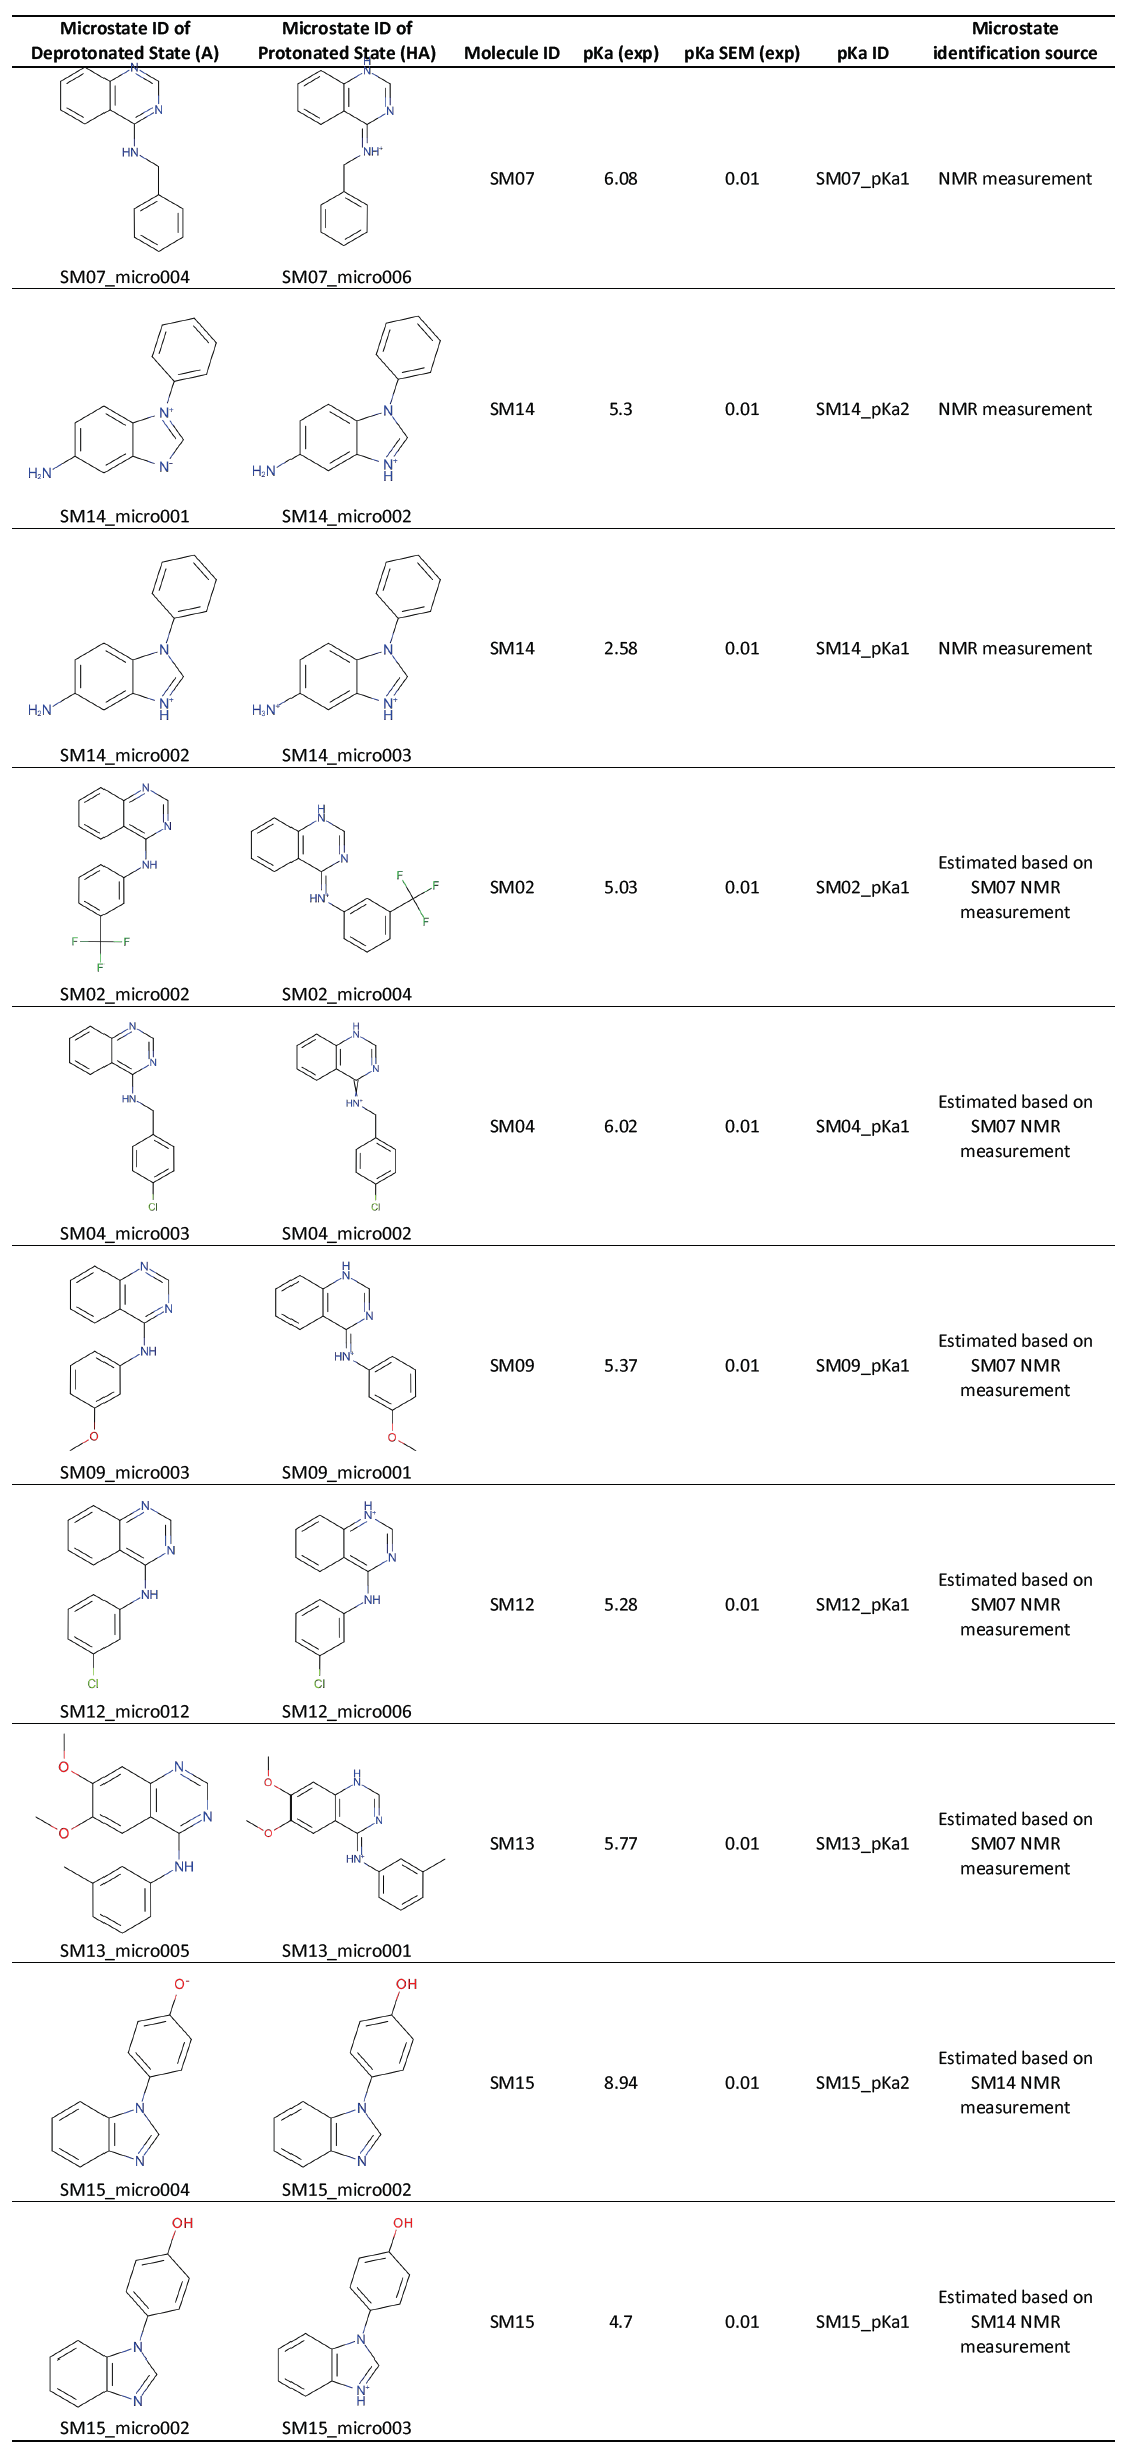
\includegraphics[width=0.5\linewidth]{figures/experimental-microstates-of-8mol-based-on-NMR.png}
\caption{ {\bf Dominant microstates of 8 molecules were determined based on NMR measurements.} Dominant microstate sequence of 6 derivatives were determined taking SM07 and SM14 as reference. Matched experimental \pKa{} values were determined by spectrophotometric \pKa{} measurements~\citep{Isik:2018:J.Comput.AidedMol.Des.}. A CSV version of this table can be found in \textit{SAMPL6-supplementary-documents.tar.gz}.
}
\label{fig:experimental-microstate-IDs-SI-table}
\end{figure}


\begin{figure}
\centering
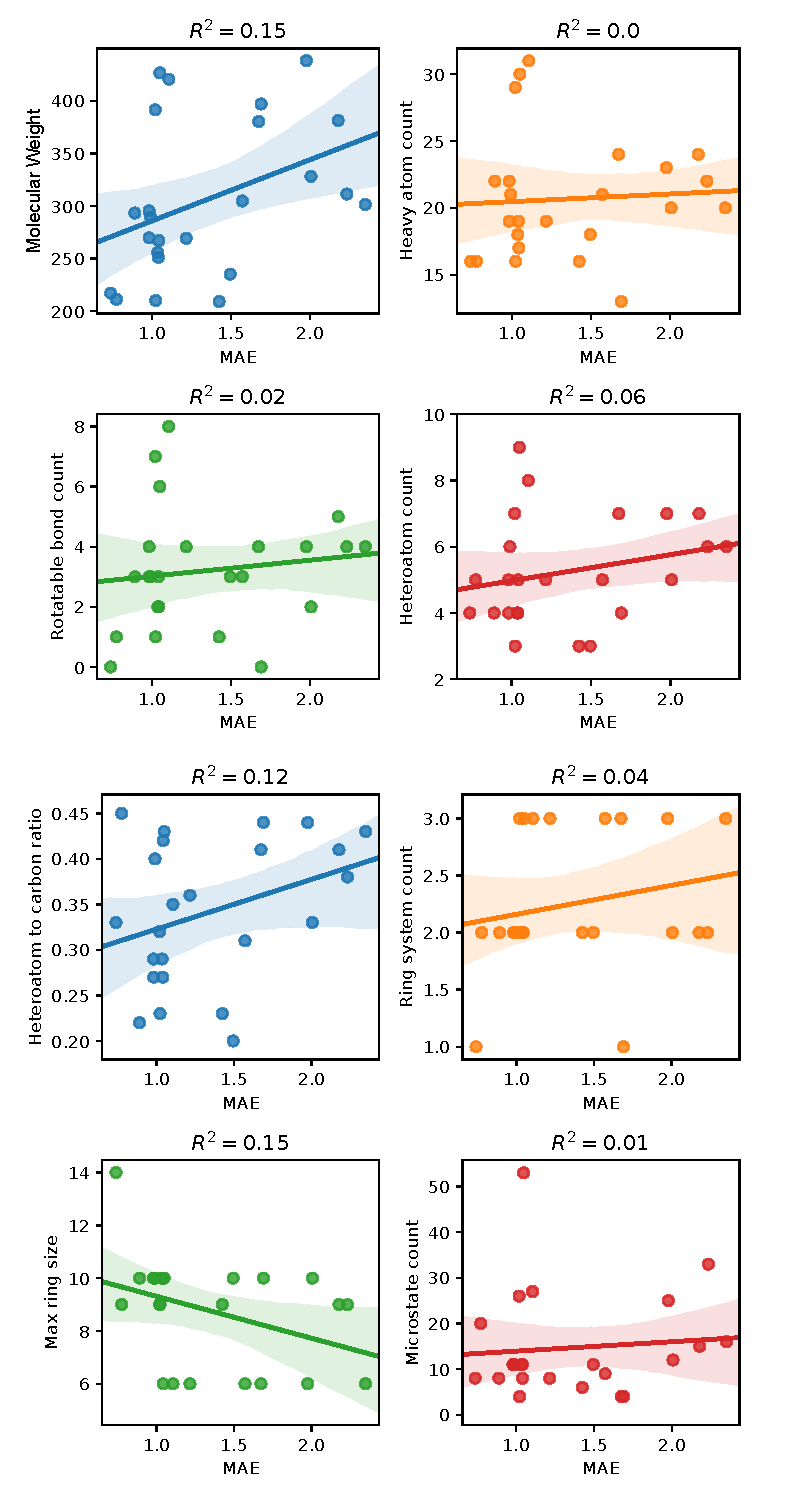
\includegraphics[width=0.5\linewidth]{figures/molecular_properties_vs_MAE_correlation_fig.pdf}
\caption{ {\bf MAE of macroscopic \pKa{} predictions of each molecule did not show any significant correlation with any molecular descriptor.} Plots show regression lines, 96\% confidence intervals of the regression lines, and R\textsubscript{2}. The following molecular descriptors were calculated using OpenEye OEMolProp Toolkit~\citep{oemolprop_openeye_2017}.
}
\label{fig:molecular_properties_vs_MAE_correlation}
\end{figure}


\begin{figure}
\centering
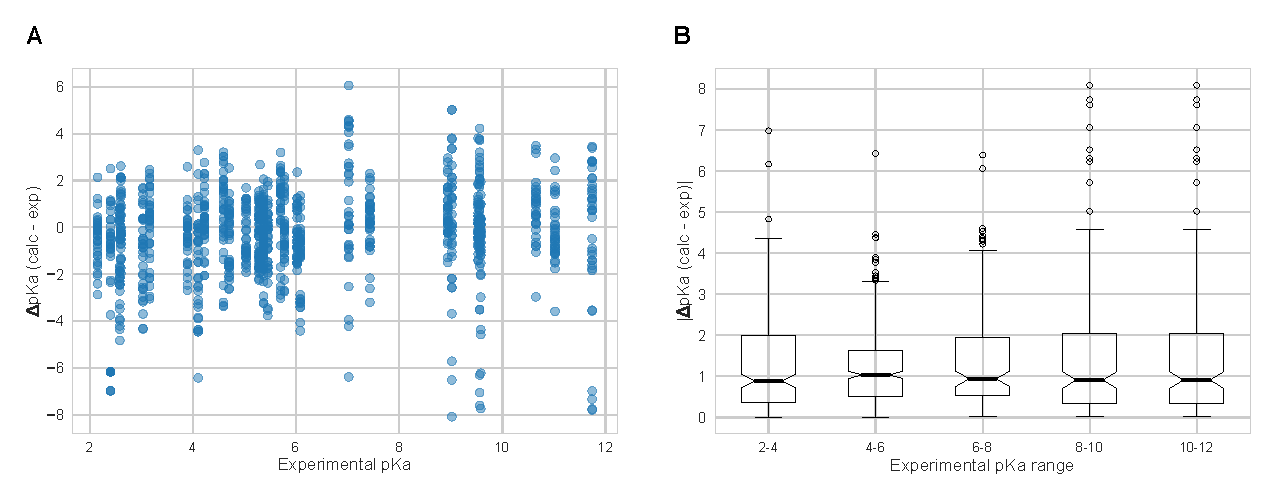
\includegraphics[width=1.0\linewidth]{figures/typeIII_error_vs_exp_pKa.pdf}
\caption{ {\bf The value of macroscopic \pKa{}s was not a factor affecting prediction error seen in SAMPL6 Challenge according to the analysis with Hungarian matching.} There was not clear trend between \pKa{} prediction error and the true \pKa{} error. Very high and very low \pKa{} values have similar inaccuracy compared to \pKa{} values close to 7. {\bf A} Scatter plot of macroscopic \pKa{} prediction error calculated with Hungarian matching vs. experimental \pKa{} value {\bf B} Box plot of absolute error of macroscopic \pKa{} predictions binned into 2 \pKa{} unit intervals of experimental \pKa{}.
}
\label{fig:macroscopic-pKa-error-vs-pKa-value}
\end{figure}


\begin{figure}
\centering
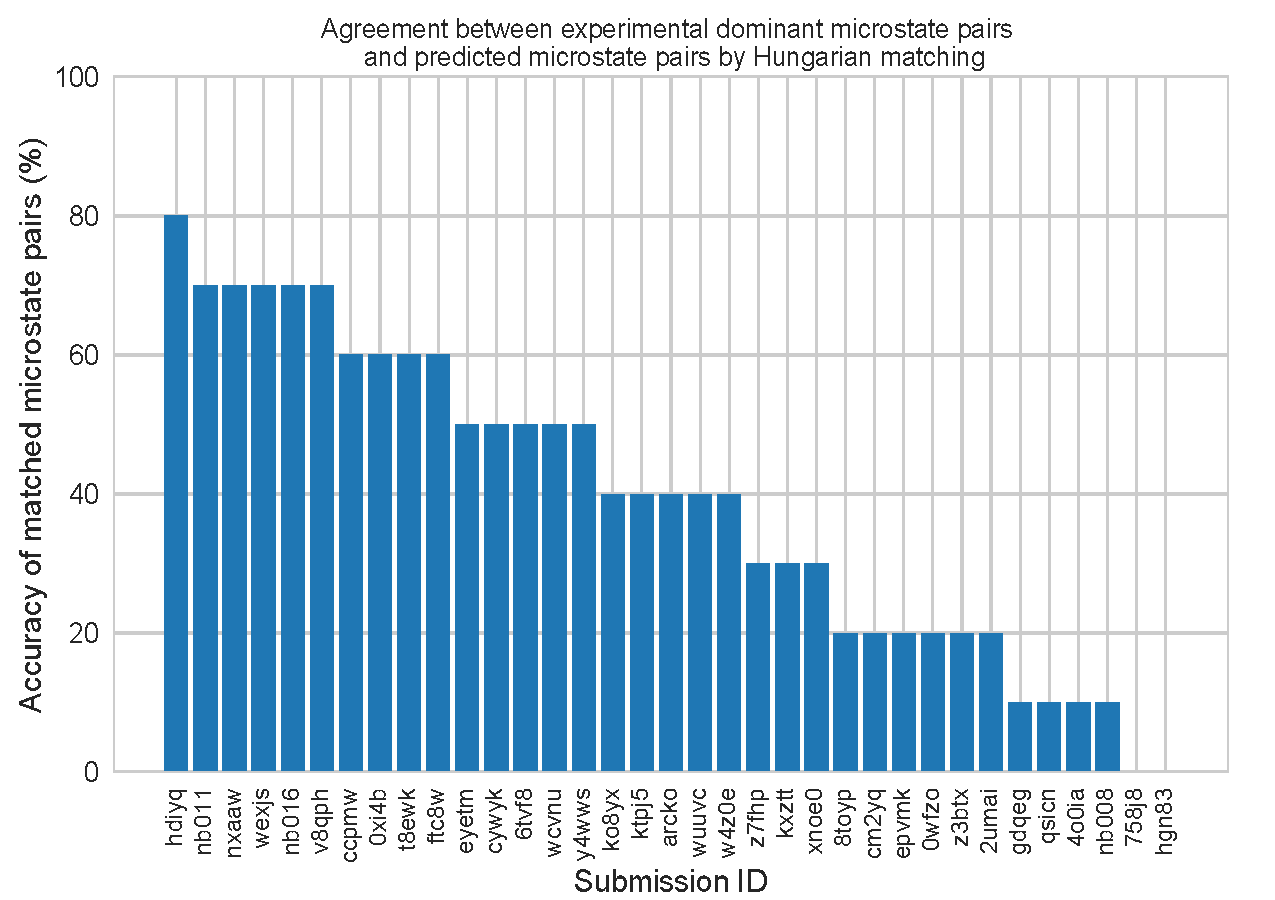
\includegraphics[width=0.75\linewidth]{figures/TypeI_Hungarian_match_microstate_pair_accuracy.pdf}
\caption{ {\bf There was low agreement between experimental dominant microstate pairs and the predicted microstate pairs selected by Hungarian algorithm for microscopic \pKa{} predictions.} This analysis could only be performed for 8 molecules with NMR data. Hungarian matching algorithm which matches predicted and experimental values considering only the closeness of the numerical value of \pKa{} and it often leds to predicted \pKa{} matches that described a different microstates pair than the experimentally observed dominant microstates..
}
\label{fig:microstate-pairs-with-Hungarian-match-vs-experiments}
\end{figure}



\end{document}
